\batchmode
\documentclass[twoside]{book}

% Packages required by doxygen
\usepackage{fixltx2e}
\usepackage{calc}
\usepackage{doxygen}
\usepackage[export]{adjustbox} % also loads graphicx
\usepackage{graphicx}
\usepackage[utf8]{inputenc}
\usepackage{makeidx}
\usepackage{multicol}
\usepackage{multirow}
\PassOptionsToPackage{warn}{textcomp}
\usepackage{textcomp}
\usepackage[nointegrals]{wasysym}
\usepackage[table]{xcolor}

% Font selection
\usepackage[T1]{fontenc}
\usepackage[scaled=.90]{helvet}
\usepackage{courier}
\usepackage{amssymb}
\usepackage{sectsty}
\renewcommand{\familydefault}{\sfdefault}
\allsectionsfont{%
  \fontseries{bc}\selectfont%
  \color{darkgray}%
}
\renewcommand{\DoxyLabelFont}{%
  \fontseries{bc}\selectfont%
  \color{darkgray}%
}
\newcommand{\+}{\discretionary{\mbox{\scriptsize$\hookleftarrow$}}{}{}}

% Page & text layout
\usepackage{geometry}
\geometry{%
  a4paper,%
  top=2.5cm,%
  bottom=2.5cm,%
  left=2.5cm,%
  right=2.5cm%
}
\tolerance=750
\hfuzz=15pt
\hbadness=750
\setlength{\emergencystretch}{15pt}
\setlength{\parindent}{0cm}
\setlength{\parskip}{3ex plus 2ex minus 2ex}
\makeatletter
\renewcommand{\paragraph}{%
  \@startsection{paragraph}{4}{0ex}{-1.0ex}{1.0ex}{%
    \normalfont\normalsize\bfseries\SS@parafont%
  }%
}
\renewcommand{\subparagraph}{%
  \@startsection{subparagraph}{5}{0ex}{-1.0ex}{1.0ex}{%
    \normalfont\normalsize\bfseries\SS@subparafont%
  }%
}
\makeatother

% Headers & footers
\usepackage{fancyhdr}
\pagestyle{fancyplain}
\fancyhead[LE]{\fancyplain{}{\bfseries\thepage}}
\fancyhead[CE]{\fancyplain{}{}}
\fancyhead[RE]{\fancyplain{}{\bfseries\leftmark}}
\fancyhead[LO]{\fancyplain{}{\bfseries\rightmark}}
\fancyhead[CO]{\fancyplain{}{}}
\fancyhead[RO]{\fancyplain{}{\bfseries\thepage}}
\fancyfoot[LE]{\fancyplain{}{}}
\fancyfoot[CE]{\fancyplain{}{}}
\fancyfoot[RE]{\fancyplain{}{\bfseries\scriptsize Generated by Doxygen }}
\fancyfoot[LO]{\fancyplain{}{\bfseries\scriptsize Generated by Doxygen }}
\fancyfoot[CO]{\fancyplain{}{}}
\fancyfoot[RO]{\fancyplain{}{}}
\renewcommand{\footrulewidth}{0.4pt}
\renewcommand{\chaptermark}[1]{%
  \markboth{#1}{}%
}
\renewcommand{\sectionmark}[1]{%
  \markright{\thesection\ #1}%
}

% Indices & bibliography
\usepackage{natbib}
\usepackage[titles]{tocloft}
\setcounter{tocdepth}{3}
\setcounter{secnumdepth}{5}
\makeindex

% Hyperlinks (required, but should be loaded last)
\usepackage{ifpdf}
\ifpdf
  \usepackage[pdftex,pagebackref=true]{hyperref}
\else
  \usepackage[ps2pdf,pagebackref=true]{hyperref}
\fi
\hypersetup{%
  colorlinks=true,%
  linkcolor=blue,%
  citecolor=blue,%
  unicode%
}

% Custom commands
\newcommand{\clearemptydoublepage}{%
  \newpage{\pagestyle{empty}\cleardoublepage}%
}

\usepackage{caption}
\captionsetup{labelsep=space,justification=centering,font={bf},singlelinecheck=off,skip=4pt,position=top}

%===== C O N T E N T S =====

\begin{document}

% Titlepage & ToC
\hypersetup{pageanchor=false,
             bookmarksnumbered=true,
             pdfencoding=unicode
            }
\pagenumbering{alph}
\pagenumbering{arabic}
\hypersetup{pageanchor=true}

%--- Begin generated contents ---
\chapter{Demo problem\+: A preconditioner for the solution of (pseudo-\/)solid mechanics problems with prescribed boundary motions}
\label{index}\hypertarget{index}{}\hypertarget{index_q}{}\section{A few quick questions...}\label{index_q}
Since {\ttfamily oomph-\/lib} is developed as open-\/source software, any evidence that the code is being downloaded and used is very helpful for us as it helps to justify our continued work on this project.

We would therefore be extremely grateful if you could provide the information requested in the form below. Pressing the \char`\"{}submit\char`\"{} button will get you to the actual download page.

{\bfseries Note\+:} 
\begin{DoxyItemize}
\item All information will be treated as confidential. 
\item If you provide your email address and check the appropriate box we will add you to our mailing list to inform you of upgrades and bug fixes to the code. Rest assured that the mailing list is {\bfseries very low volume} -- we have better things to do than to bombard you with email. 
\item If you still feel reluctant to provide any of the information requested, feel free to enter some dummy input. The form will check that {\bfseries some} information has been entered but entering your name as \char`\"{}\+Joe Cool\char`\"{} is perfectly acceptable -- this is to discourage people from not providing the information simply because they are too lazy to type... 
\end{DoxyItemize}



 







 

 \hypertarget{index_pdf}{}\section{P\+D\+F file}\label{index_pdf}
A \href{../latex/refman.pdf}{\tt pdf version} of this document is available. \end{document}

\chapter{Namespace Index}
\section{Namespace List}
Here is a list of all namespaces with brief descriptions\+:\begin{DoxyCompactList}
\item\contentsline{section}{\hyperlink{namespaceGlobal__Physical__Variables}{Global\+\_\+\+Physical\+\_\+\+Variables} \\*Global variables that represent physical properties }{\pageref{namespaceGlobal__Physical__Variables}}{}
\item\contentsline{section}{\hyperlink{namespaceoomph}{oomph} }{\pageref{namespaceoomph}}{}
\item\contentsline{section}{\hyperlink{namespacePhysical__Variables}{Physical\+\_\+\+Variables} \\*Namespace for the solution of 2D linear shell equation }{\pageref{namespacePhysical__Variables}}{}
\end{DoxyCompactList}

\chapter{Hierarchical Index}
\section{Class Hierarchy}
This inheritance list is sorted roughly, but not completely, alphabetically\+:\begin{DoxyCompactList}
\item Problem\begin{DoxyCompactList}
\item \contentsline{section}{Unstructured\+Solid\+Problem$<$ E\+L\+E\+M\+E\+NT $>$}{\pageref{classUnstructuredSolidProblem}}{}
\end{DoxyCompactList}
\end{DoxyCompactList}

\chapter{Class Index}
\section{Class List}
Here are the classes, structs, unions and interfaces with brief descriptions\+:\begin{DoxyCompactList}
\item\contentsline{section}{\hyperlink{classPMLProblem}{P\+M\+L\+Problem$<$ E\+L\+E\+M\+E\+N\+T $>$} }{\pageref{classPMLProblem}}{}
\item\contentsline{section}{\hyperlink{classGlobalParameters_1_1TestPMLMapping}{Global\+Parameters\+::\+Test\+P\+M\+L\+Mapping} }{\pageref{classGlobalParameters_1_1TestPMLMapping}}{}
\end{DoxyCompactList}

\chapter{File Index}
\section{File List}
Here is a list of all files with brief descriptions\+:\begin{DoxyCompactList}
\item\contentsline{section}{\hyperlink{jeffery__orbit_8cc}{jeffery\+\_\+orbit.\+cc} }{\pageref{jeffery__orbit_8cc}}{}
\item\contentsline{section}{\hyperlink{jeffery__orbit_8txt__doxygenified_8h}{jeffery\+\_\+orbit.\+txt\+\_\+doxygenified.\+h} }{\pageref{jeffery__orbit_8txt__doxygenified_8h}}{}
\item\contentsline{section}{\hyperlink{my__taylor__hood__elements_8h}{my\+\_\+taylor\+\_\+hood\+\_\+elements.\+h} }{\pageref{my__taylor__hood__elements_8h}}{}
\end{DoxyCompactList}

\chapter{Namespace Documentation}
\hypertarget{namespaceDiagonalPreconditionerHelper}{}\section{Diagonal\+Preconditioner\+Helper Namespace Reference}
\label{namespaceDiagonalPreconditionerHelper}\index{Diagonal\+Preconditioner\+Helper@{Diagonal\+Preconditioner\+Helper}}
\subsection*{Functions}
\begin{DoxyCompactItemize}
\item 
Preconditioner $\ast$ \hyperlink{namespaceDiagonalPreconditionerHelper_a455a8314b4dc41c20c9859b8509cc740}{get\+\_\+diagonal\+\_\+preconditioner} ()
\begin{DoxyCompactList}\small\item\em Create a matrix-\/based diagonal preconditioner for subsidiary linear systems. \end{DoxyCompactList}\end{DoxyCompactItemize}


\subsection{Detailed Description}
Namespace to \char`\"{}hide\char`\"{} global function that creates an instance of oomph-\/lib\textquotesingle{}s diagonal preconditioner. 

\subsection{Function Documentation}
\mbox{\Hypertarget{namespaceDiagonalPreconditionerHelper_a455a8314b4dc41c20c9859b8509cc740}\label{namespaceDiagonalPreconditionerHelper_a455a8314b4dc41c20c9859b8509cc740}} 
\index{Diagonal\+Preconditioner\+Helper@{Diagonal\+Preconditioner\+Helper}!get\+\_\+diagonal\+\_\+preconditioner@{get\+\_\+diagonal\+\_\+preconditioner}}
\index{get\+\_\+diagonal\+\_\+preconditioner@{get\+\_\+diagonal\+\_\+preconditioner}!Diagonal\+Preconditioner\+Helper@{Diagonal\+Preconditioner\+Helper}}
\subsubsection{\texorpdfstring{get\+\_\+diagonal\+\_\+preconditioner()}{get\_diagonal\_preconditioner()}}
{\footnotesize\ttfamily Preconditioner$\ast$ Diagonal\+Preconditioner\+Helper\+::get\+\_\+diagonal\+\_\+preconditioner (\begin{DoxyParamCaption}{ }\end{DoxyParamCaption})}



Create a matrix-\/based diagonal preconditioner for subsidiary linear systems. 



Definition at line 178 of file prescribed\+\_\+displ\+\_\+lagr\+\_\+mult\+\_\+precond.\+cc.



Referenced by Prescribed\+Boundary\+Displacement\+Problem$<$ E\+L\+E\+M\+E\+N\+T $>$\+::\+Prescribed\+Boundary\+Displacement\+Problem().


\hypertarget{namespaceGlobal__Physical__Variables}{}\section{Global\+\_\+\+Physical\+\_\+\+Variables Namespace Reference}
\label{namespaceGlobal__Physical__Variables}\index{Global\+\_\+\+Physical\+\_\+\+Variables@{Global\+\_\+\+Physical\+\_\+\+Variables}}


Namespace for physical parameters.  


\subsection*{Functions}
\begin{DoxyCompactItemize}
\item 
Vector$<$ double $>$ \hyperlink{namespaceGlobal__Physical__Variables_afae321364975eb56688ad13abc8ed6b7}{Gravity} (2)
\begin{DoxyCompactList}\small\item\em Gravity vector. \end{DoxyCompactList}\item 
void \hyperlink{namespaceGlobal__Physical__Variables_a87da705b8a46bed337cf5dbdd788b87b}{body\+\_\+force} (const double \&time, const Vector$<$ double $>$ \&x, Vector$<$ double $>$ \&result)
\begin{DoxyCompactList}\small\item\em Functional body force. \end{DoxyCompactList}\item 
void \hyperlink{namespaceGlobal__Physical__Variables_a9780d615ae07c4e00a436ab2973b54e6}{zero\+\_\+body\+\_\+force} (const double \&time, const Vector$<$ double $>$ \&x, Vector$<$ double $>$ \&result)
\begin{DoxyCompactList}\small\item\em Zero functional body force. \end{DoxyCompactList}\end{DoxyCompactItemize}
\subsection*{Variables}
\begin{DoxyCompactItemize}
\item 
double \hyperlink{namespaceGlobal__Physical__Variables_ab814e627d2eb5bc50318879d19ab16b9}{Re} =100
\begin{DoxyCompactList}\small\item\em Reynolds number. \end{DoxyCompactList}\item 
double \hyperlink{namespaceGlobal__Physical__Variables_ab1a845a672b4d74b304639a976dc65c6}{Re\+\_\+inv\+Fr} =100
\begin{DoxyCompactList}\small\item\em Reynolds/\+Froude number. \end{DoxyCompactList}\end{DoxyCompactItemize}


\subsection{Detailed Description}
Namespace for physical parameters. 

\subsection{Function Documentation}
\mbox{\Hypertarget{namespaceGlobal__Physical__Variables_a87da705b8a46bed337cf5dbdd788b87b}\label{namespaceGlobal__Physical__Variables_a87da705b8a46bed337cf5dbdd788b87b}} 
\index{Global\+\_\+\+Physical\+\_\+\+Variables@{Global\+\_\+\+Physical\+\_\+\+Variables}!body\+\_\+force@{body\+\_\+force}}
\index{body\+\_\+force@{body\+\_\+force}!Global\+\_\+\+Physical\+\_\+\+Variables@{Global\+\_\+\+Physical\+\_\+\+Variables}}
\subsubsection{\texorpdfstring{body\+\_\+force()}{body\_force()}}
{\footnotesize\ttfamily void Global\+\_\+\+Physical\+\_\+\+Variables\+::body\+\_\+force (\begin{DoxyParamCaption}\item[{const double \&}]{time,  }\item[{const Vector$<$ double $>$ \&}]{x,  }\item[{Vector$<$ double $>$ \&}]{result }\end{DoxyParamCaption})}



Functional body force. 



Definition at line 62 of file circular\+\_\+driven\+\_\+cavity.\+cc.



References Re\+\_\+inv\+Fr.



Referenced by main().

\mbox{\Hypertarget{namespaceGlobal__Physical__Variables_afae321364975eb56688ad13abc8ed6b7}\label{namespaceGlobal__Physical__Variables_afae321364975eb56688ad13abc8ed6b7}} 
\index{Global\+\_\+\+Physical\+\_\+\+Variables@{Global\+\_\+\+Physical\+\_\+\+Variables}!Gravity@{Gravity}}
\index{Gravity@{Gravity}!Global\+\_\+\+Physical\+\_\+\+Variables@{Global\+\_\+\+Physical\+\_\+\+Variables}}
\subsubsection{\texorpdfstring{Gravity()}{Gravity()}}
{\footnotesize\ttfamily Vector$<$double$>$ Global\+\_\+\+Physical\+\_\+\+Variables\+::\+Gravity (\begin{DoxyParamCaption}\item[{2}]{ }\end{DoxyParamCaption})}



Gravity vector. 



Referenced by main(), and Quarter\+Circle\+Driven\+Cavity\+Problem$<$ E\+L\+E\+M\+E\+N\+T $>$\+::\+Quarter\+Circle\+Driven\+Cavity\+Problem().

\mbox{\Hypertarget{namespaceGlobal__Physical__Variables_a9780d615ae07c4e00a436ab2973b54e6}\label{namespaceGlobal__Physical__Variables_a9780d615ae07c4e00a436ab2973b54e6}} 
\index{Global\+\_\+\+Physical\+\_\+\+Variables@{Global\+\_\+\+Physical\+\_\+\+Variables}!zero\+\_\+body\+\_\+force@{zero\+\_\+body\+\_\+force}}
\index{zero\+\_\+body\+\_\+force@{zero\+\_\+body\+\_\+force}!Global\+\_\+\+Physical\+\_\+\+Variables@{Global\+\_\+\+Physical\+\_\+\+Variables}}
\subsubsection{\texorpdfstring{zero\+\_\+body\+\_\+force()}{zero\_body\_force()}}
{\footnotesize\ttfamily void Global\+\_\+\+Physical\+\_\+\+Variables\+::zero\+\_\+body\+\_\+force (\begin{DoxyParamCaption}\item[{const double \&}]{time,  }\item[{const Vector$<$ double $>$ \&}]{x,  }\item[{Vector$<$ double $>$ \&}]{result }\end{DoxyParamCaption})}



Zero functional body force. 



Definition at line 70 of file circular\+\_\+driven\+\_\+cavity.\+cc.



Referenced by main().



\subsection{Variable Documentation}
\mbox{\Hypertarget{namespaceGlobal__Physical__Variables_ab814e627d2eb5bc50318879d19ab16b9}\label{namespaceGlobal__Physical__Variables_ab814e627d2eb5bc50318879d19ab16b9}} 
\index{Global\+\_\+\+Physical\+\_\+\+Variables@{Global\+\_\+\+Physical\+\_\+\+Variables}!Re@{Re}}
\index{Re@{Re}!Global\+\_\+\+Physical\+\_\+\+Variables@{Global\+\_\+\+Physical\+\_\+\+Variables}}
\subsubsection{\texorpdfstring{Re}{Re}}
{\footnotesize\ttfamily double Global\+\_\+\+Physical\+\_\+\+Variables\+::\+Re =100}



Reynolds number. 



Definition at line 53 of file circular\+\_\+driven\+\_\+cavity.\+cc.



Referenced by Quarter\+Circle\+Driven\+Cavity\+Problem$<$ E\+L\+E\+M\+E\+N\+T $>$\+::\+Quarter\+Circle\+Driven\+Cavity\+Problem().

\mbox{\Hypertarget{namespaceGlobal__Physical__Variables_ab1a845a672b4d74b304639a976dc65c6}\label{namespaceGlobal__Physical__Variables_ab1a845a672b4d74b304639a976dc65c6}} 
\index{Global\+\_\+\+Physical\+\_\+\+Variables@{Global\+\_\+\+Physical\+\_\+\+Variables}!Re\+\_\+inv\+Fr@{Re\+\_\+inv\+Fr}}
\index{Re\+\_\+inv\+Fr@{Re\+\_\+inv\+Fr}!Global\+\_\+\+Physical\+\_\+\+Variables@{Global\+\_\+\+Physical\+\_\+\+Variables}}
\subsubsection{\texorpdfstring{Re\+\_\+inv\+Fr}{Re\_invFr}}
{\footnotesize\ttfamily double Global\+\_\+\+Physical\+\_\+\+Variables\+::\+Re\+\_\+inv\+Fr =100}



Reynolds/\+Froude number. 



Definition at line 56 of file circular\+\_\+driven\+\_\+cavity.\+cc.



Referenced by body\+\_\+force(), and Quarter\+Circle\+Driven\+Cavity\+Problem$<$ E\+L\+E\+M\+E\+N\+T $>$\+::\+Quarter\+Circle\+Driven\+Cavity\+Problem().


\hypertarget{namespaceoomph}{}\section{oomph Namespace Reference}
\label{namespaceoomph}\index{oomph@{oomph}}
\subsection*{Classes}
\begin{DoxyCompactItemize}
\item 
class \hyperlink{classoomph_1_1BellShellElement}{Bell\+Shell\+Element}
\begin{DoxyCompactList}\small\item\em \hyperlink{classoomph_1_1BellShellElement}{Bell\+Shell\+Element} elements are with subparametric interpolation for the function. \end{DoxyCompactList}\item 
class \hyperlink{classoomph_1_1FaceGeometry_3_01BellShellElement_3_01DIM_00_01NNODE__1D_01_4_01_4}{Face\+Geometry$<$ Bell\+Shell\+Element$<$ D\+I\+M, N\+N\+O\+D\+E\+\_\+1\+D $>$ $>$}
\item 
class \hyperlink{classoomph_1_1MyShellEquations}{My\+Shell\+Equations}
\item 
class \hyperlink{classoomph_1_1Plate}{Plate}
\begin{DoxyCompactList}\small\item\em Elliptical tube with half axes a and b. \end{DoxyCompactList}\end{DoxyCompactItemize}

\chapter{Class Documentation}
\hypertarget{classoomph_1_1FaceGeometry_3_01PseudoElasticBulkElement_3_01ELEMENT_01_4_01_4}{}\section{oomph\+:\+:Face\+Geometry$<$ Pseudo\+Elastic\+Bulk\+Element$<$ E\+L\+E\+M\+E\+NT $>$ $>$ Class Template Reference}
\label{classoomph_1_1FaceGeometry_3_01PseudoElasticBulkElement_3_01ELEMENT_01_4_01_4}\index{oomph\+::\+Face\+Geometry$<$ Pseudo\+Elastic\+Bulk\+Element$<$ E\+L\+E\+M\+E\+N\+T $>$ $>$@{oomph\+::\+Face\+Geometry$<$ Pseudo\+Elastic\+Bulk\+Element$<$ E\+L\+E\+M\+E\+N\+T $>$ $>$}}


Face\+Geometry of wrapped element is the same as the underlying element.  


Inheritance diagram for oomph\+:\+:Face\+Geometry$<$ Pseudo\+Elastic\+Bulk\+Element$<$ E\+L\+E\+M\+E\+NT $>$ $>$\+:\begin{figure}[H]
\begin{center}
\leavevmode
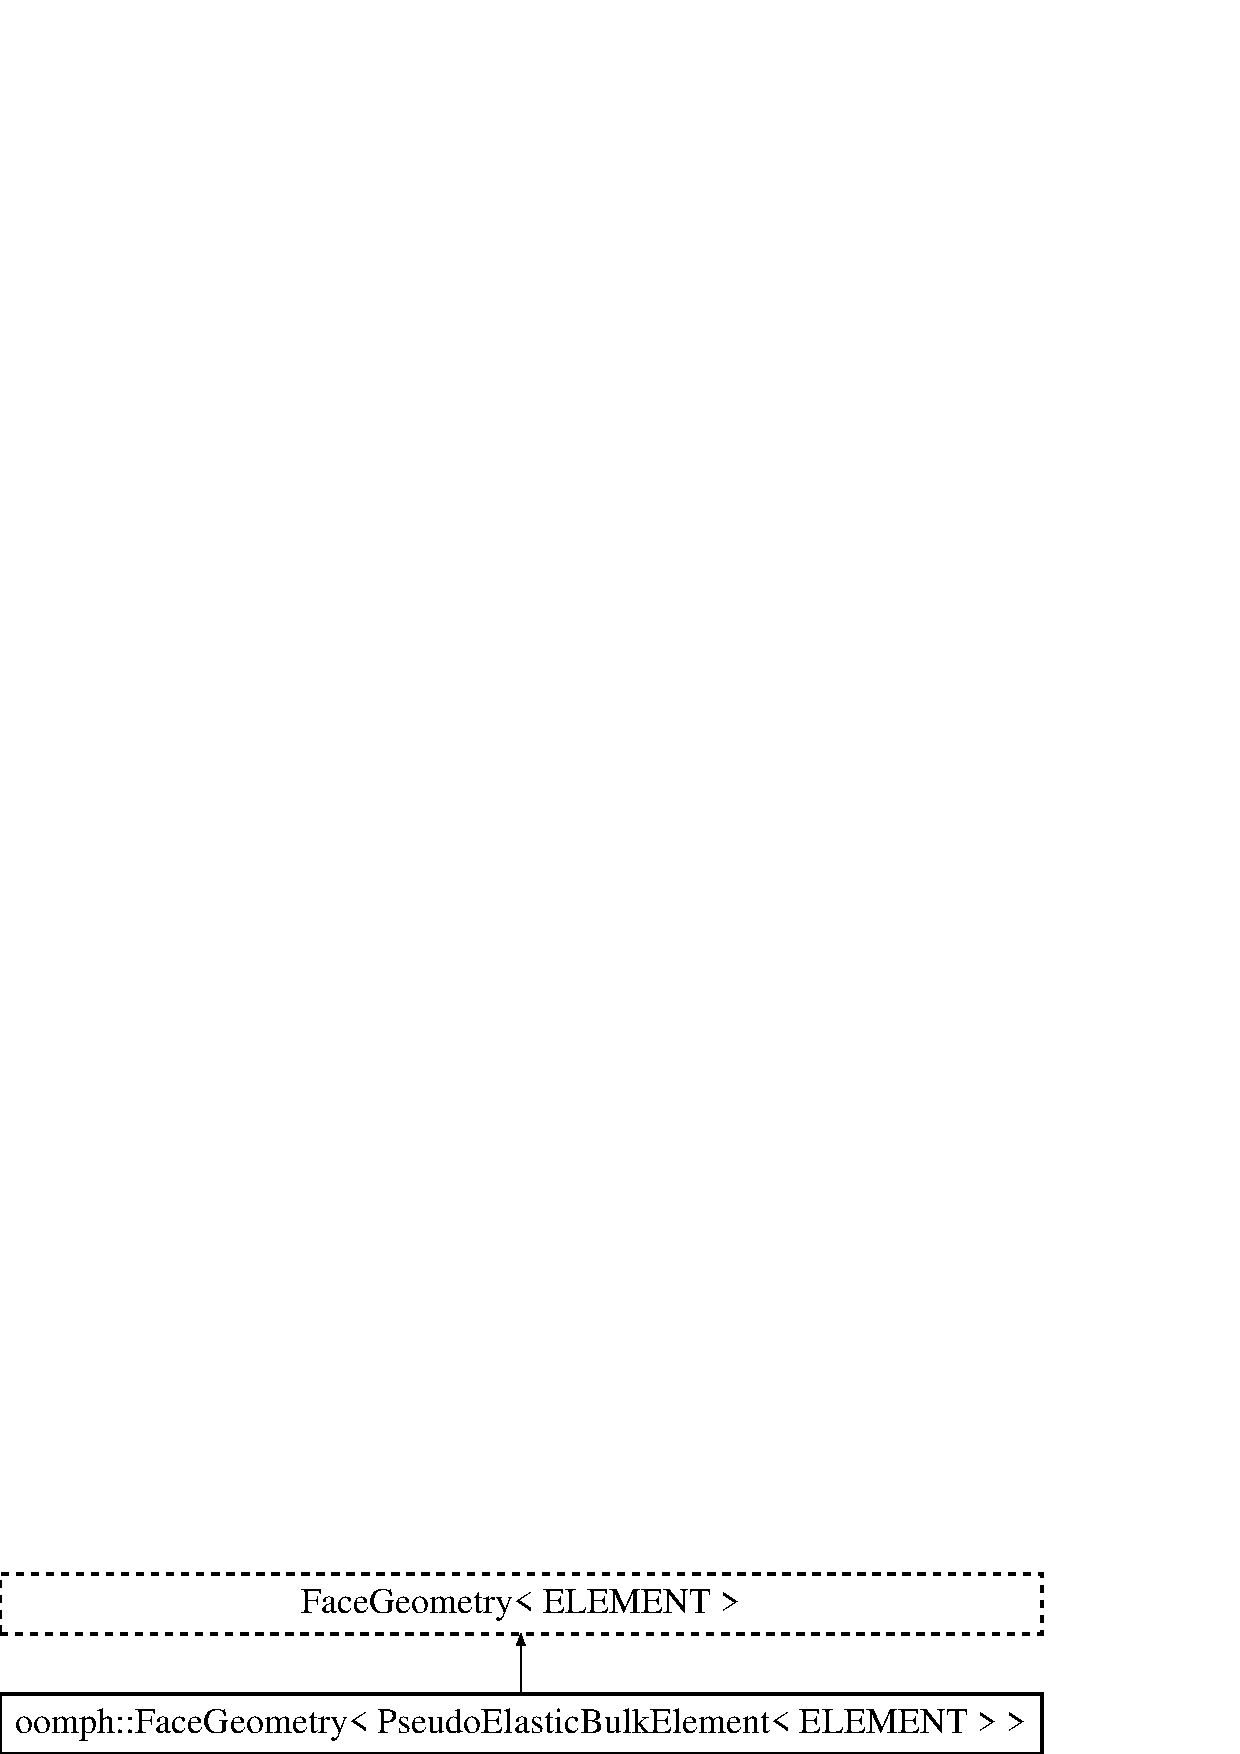
\includegraphics[height=2.000000cm]{classoomph_1_1FaceGeometry_3_01PseudoElasticBulkElement_3_01ELEMENT_01_4_01_4}
\end{center}
\end{figure}
\subsection*{Public Member Functions}
\begin{DoxyCompactItemize}
\item 
\hyperlink{classoomph_1_1FaceGeometry_3_01PseudoElasticBulkElement_3_01ELEMENT_01_4_01_4_a3f79ef40a41543c9d96ef84aecc202f3}{Face\+Geometry} ()
\begin{DoxyCompactList}\small\item\em Constructor -- required for more recent versions of gcc. \end{DoxyCompactList}\end{DoxyCompactItemize}


\subsection{Detailed Description}
\subsubsection*{template$<$class E\+L\+E\+M\+E\+NT$>$\newline
class oomph\+::\+Face\+Geometry$<$ Pseudo\+Elastic\+Bulk\+Element$<$ E\+L\+E\+M\+E\+N\+T $>$ $>$}

Face\+Geometry of wrapped element is the same as the underlying element. 

Definition at line 145 of file prescribed\+\_\+displ\+\_\+lagr\+\_\+mult\+\_\+precond.\+cc.



\subsection{Constructor \& Destructor Documentation}
\mbox{\Hypertarget{classoomph_1_1FaceGeometry_3_01PseudoElasticBulkElement_3_01ELEMENT_01_4_01_4_a3f79ef40a41543c9d96ef84aecc202f3}\label{classoomph_1_1FaceGeometry_3_01PseudoElasticBulkElement_3_01ELEMENT_01_4_01_4_a3f79ef40a41543c9d96ef84aecc202f3}} 
\index{oomph\+::\+Face\+Geometry$<$ Pseudo\+Elastic\+Bulk\+Element$<$ E\+L\+E\+M\+E\+N\+T $>$ $>$@{oomph\+::\+Face\+Geometry$<$ Pseudo\+Elastic\+Bulk\+Element$<$ E\+L\+E\+M\+E\+N\+T $>$ $>$}!Face\+Geometry@{Face\+Geometry}}
\index{Face\+Geometry@{Face\+Geometry}!oomph\+::\+Face\+Geometry$<$ Pseudo\+Elastic\+Bulk\+Element$<$ E\+L\+E\+M\+E\+N\+T $>$ $>$@{oomph\+::\+Face\+Geometry$<$ Pseudo\+Elastic\+Bulk\+Element$<$ E\+L\+E\+M\+E\+N\+T $>$ $>$}}
\subsubsection{\texorpdfstring{Face\+Geometry()}{FaceGeometry()}}
{\footnotesize\ttfamily template$<$class E\+L\+E\+M\+E\+NT $>$ \\
oomph\+::\+Face\+Geometry$<$ \hyperlink{classoomph_1_1PseudoElasticBulkElement}{Pseudo\+Elastic\+Bulk\+Element}$<$ E\+L\+E\+M\+E\+NT $>$ $>$\+::Face\+Geometry (\begin{DoxyParamCaption}{ }\end{DoxyParamCaption})\hspace{0.3cm}{\ttfamily [inline]}}



Constructor -- required for more recent versions of gcc. 



Definition at line 152 of file prescribed\+\_\+displ\+\_\+lagr\+\_\+mult\+\_\+precond.\+cc.



The documentation for this class was generated from the following file\+:\begin{DoxyCompactItemize}
\item 
\hyperlink{prescribed__displ__lagr__mult__precond_8cc}{prescribed\+\_\+displ\+\_\+lagr\+\_\+mult\+\_\+precond.\+cc}\end{DoxyCompactItemize}

\hypertarget{classFiniteElementComp}{}\section{Finite\+Element\+Comp Class Reference}
\label{classFiniteElementComp}\index{Finite\+Element\+Comp@{Finite\+Element\+Comp}}
\subsection*{Public Member Functions}
\begin{DoxyCompactItemize}
\item 
bool \hyperlink{classFiniteElementComp_a23bc6293da4cbec67f9e43653778440f}{operator()} (Finite\+Element $\ast$const \&el1\+\_\+pt, Finite\+Element $\ast$const \&el2\+\_\+pt) const
\begin{DoxyCompactList}\small\item\em Comparison. Is x coordinate of el1\+\_\+pt less than that of el2\+\_\+pt? \end{DoxyCompactList}\item 
bool \hyperlink{classFiniteElementComp_a23bc6293da4cbec67f9e43653778440f}{operator()} (Finite\+Element $\ast$const \&el1\+\_\+pt, Finite\+Element $\ast$const \&el2\+\_\+pt) const
\begin{DoxyCompactList}\small\item\em Comparison. Is x coordinate of el1\+\_\+pt less than that of el2\+\_\+pt? \end{DoxyCompactList}\end{DoxyCompactItemize}


\subsection{Detailed Description}
Function-\/type-\/object to compare finite elements based on their x coordinate 

Definition at line 51 of file prescribed\+\_\+displ\+\_\+lagr\+\_\+mult.\+cc.



\subsection{Member Function Documentation}
\mbox{\Hypertarget{classFiniteElementComp_a23bc6293da4cbec67f9e43653778440f}\label{classFiniteElementComp_a23bc6293da4cbec67f9e43653778440f}} 
\index{Finite\+Element\+Comp@{Finite\+Element\+Comp}!operator()@{operator()}}
\index{operator()@{operator()}!Finite\+Element\+Comp@{Finite\+Element\+Comp}}
\subsubsection{\texorpdfstring{operator()()}{operator()()}\hspace{0.1cm}{\footnotesize\ttfamily [1/2]}}
{\footnotesize\ttfamily bool Finite\+Element\+Comp\+::operator() (\begin{DoxyParamCaption}\item[{Finite\+Element $\ast$const \&}]{el1\+\_\+pt,  }\item[{Finite\+Element $\ast$const \&}]{el2\+\_\+pt }\end{DoxyParamCaption}) const\hspace{0.3cm}{\ttfamily [inline]}}



Comparison. Is x coordinate of el1\+\_\+pt less than that of el2\+\_\+pt? 



Definition at line 57 of file prescribed\+\_\+displ\+\_\+lagr\+\_\+mult.\+cc.

\mbox{\Hypertarget{classFiniteElementComp_a23bc6293da4cbec67f9e43653778440f}\label{classFiniteElementComp_a23bc6293da4cbec67f9e43653778440f}} 
\index{Finite\+Element\+Comp@{Finite\+Element\+Comp}!operator()@{operator()}}
\index{operator()@{operator()}!Finite\+Element\+Comp@{Finite\+Element\+Comp}}
\subsubsection{\texorpdfstring{operator()()}{operator()()}\hspace{0.1cm}{\footnotesize\ttfamily [2/2]}}
{\footnotesize\ttfamily bool Finite\+Element\+Comp\+::operator() (\begin{DoxyParamCaption}\item[{Finite\+Element $\ast$const \&}]{el1\+\_\+pt,  }\item[{Finite\+Element $\ast$const \&}]{el2\+\_\+pt }\end{DoxyParamCaption}) const\hspace{0.3cm}{\ttfamily [inline]}}



Comparison. Is x coordinate of el1\+\_\+pt less than that of el2\+\_\+pt? 



Definition at line 204 of file prescribed\+\_\+displ\+\_\+lagr\+\_\+mult\+\_\+precond.\+cc.



The documentation for this class was generated from the following files\+:\begin{DoxyCompactItemize}
\item 
\hyperlink{prescribed__displ__lagr__mult_8cc}{prescribed\+\_\+displ\+\_\+lagr\+\_\+mult.\+cc}\item 
\hyperlink{prescribed__displ__lagr__mult__precond_8cc}{prescribed\+\_\+displ\+\_\+lagr\+\_\+mult\+\_\+precond.\+cc}\end{DoxyCompactItemize}

\hypertarget{classPrescribedBoundaryDisplacementProblem}{}\section{Prescribed\+Boundary\+Displacement\+Problem$<$ E\+L\+E\+M\+E\+NT $>$ Class Template Reference}
\label{classPrescribedBoundaryDisplacementProblem}\index{Prescribed\+Boundary\+Displacement\+Problem$<$ E\+L\+E\+M\+E\+N\+T $>$@{Prescribed\+Boundary\+Displacement\+Problem$<$ E\+L\+E\+M\+E\+N\+T $>$}}
Inheritance diagram for Prescribed\+Boundary\+Displacement\+Problem$<$ E\+L\+E\+M\+E\+NT $>$\+:\begin{figure}[H]
\begin{center}
\leavevmode
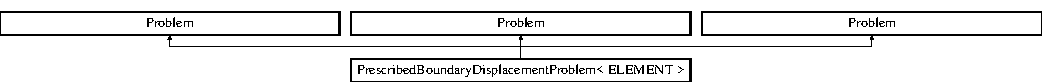
\includegraphics[height=1.098039cm]{classPrescribedBoundaryDisplacementProblem}
\end{center}
\end{figure}
\subsection*{Public Member Functions}
\begin{DoxyCompactItemize}
\item 
\hyperlink{classPrescribedBoundaryDisplacementProblem_ac0c8b47eeb75ba2c618757e6b56e62dc}{Prescribed\+Boundary\+Displacement\+Problem} ()
\begin{DoxyCompactList}\small\item\em Constructor\+: \end{DoxyCompactList}\item 
void \hyperlink{classPrescribedBoundaryDisplacementProblem_a53e7d18d9d748388160d6c4106f1d493}{actions\+\_\+after\+\_\+newton\+\_\+solve} ()
\begin{DoxyCompactList}\small\item\em Update function (empty) \end{DoxyCompactList}\item 
void \hyperlink{classPrescribedBoundaryDisplacementProblem_ad2184bb8d7391da21bec62d4aacf5c20}{actions\+\_\+before\+\_\+newton\+\_\+solve} ()
\begin{DoxyCompactList}\small\item\em Update function (empty) \end{DoxyCompactList}\item 
Elastic\+Refineable\+Rectangular\+Quad\+Mesh$<$ E\+L\+E\+M\+E\+NT $>$ $\ast$\& \hyperlink{classPrescribedBoundaryDisplacementProblem_ac0fc3028f61cec5ac4b01670d7728934}{solid\+\_\+mesh\+\_\+pt} ()
\begin{DoxyCompactList}\small\item\em Access function for the solid mesh. \end{DoxyCompactList}\item 
void \hyperlink{classPrescribedBoundaryDisplacementProblem_a2e9f335e8680b0f2338b579e37e9d38a}{actions\+\_\+before\+\_\+adapt} ()
\begin{DoxyCompactList}\small\item\em Actions before adapt\+: Wipe the mesh of Lagrange multiplier elements. \end{DoxyCompactList}\item 
void \hyperlink{classPrescribedBoundaryDisplacementProblem_aae7225db18ad5c8429c0eb96fa37b585}{actions\+\_\+after\+\_\+adapt} ()
\begin{DoxyCompactList}\small\item\em Actions after adapt\+: Rebuild the mesh of Lagrange multiplier elements. \end{DoxyCompactList}\item 
void \hyperlink{classPrescribedBoundaryDisplacementProblem_abc58821d6b49cd9773dcd90b240aab6e}{doc\+\_\+solution} ()
\begin{DoxyCompactList}\small\item\em Doc the solution. \end{DoxyCompactList}\item 
\hyperlink{classPrescribedBoundaryDisplacementProblem_ac0c8b47eeb75ba2c618757e6b56e62dc}{Prescribed\+Boundary\+Displacement\+Problem} ()
\begin{DoxyCompactList}\small\item\em Constructor\+: \end{DoxyCompactList}\item 
void \hyperlink{classPrescribedBoundaryDisplacementProblem_a53e7d18d9d748388160d6c4106f1d493}{actions\+\_\+after\+\_\+newton\+\_\+solve} ()
\begin{DoxyCompactList}\small\item\em Update function (empty) \end{DoxyCompactList}\item 
void \hyperlink{classPrescribedBoundaryDisplacementProblem_ad2184bb8d7391da21bec62d4aacf5c20}{actions\+\_\+before\+\_\+newton\+\_\+solve} ()
\begin{DoxyCompactList}\small\item\em Update boundary position directly. \end{DoxyCompactList}\item 
Elastic\+Refineable\+Rectangular\+Quad\+Mesh$<$ E\+L\+E\+M\+E\+NT $>$ $\ast$\& \hyperlink{classPrescribedBoundaryDisplacementProblem_ac0fc3028f61cec5ac4b01670d7728934}{solid\+\_\+mesh\+\_\+pt} ()
\begin{DoxyCompactList}\small\item\em Access function for the solid mesh. \end{DoxyCompactList}\item 
void \hyperlink{classPrescribedBoundaryDisplacementProblem_aae7225db18ad5c8429c0eb96fa37b585}{actions\+\_\+after\+\_\+adapt} ()
\begin{DoxyCompactList}\small\item\em Actions after adapt\+: Pin the redundant solid pressures (if any) \end{DoxyCompactList}\item 
void \hyperlink{classPrescribedBoundaryDisplacementProblem_abc58821d6b49cd9773dcd90b240aab6e}{doc\+\_\+solution} ()
\begin{DoxyCompactList}\small\item\em Doc the solution. \end{DoxyCompactList}\item 
\hyperlink{classPrescribedBoundaryDisplacementProblem_a7b5c8949e774e0ac46ddc6481e9d96df}{Prescribed\+Boundary\+Displacement\+Problem} (const unsigned \&nel\+\_\+1d)
\begin{DoxyCompactList}\small\item\em Constructor\+: Pass in number of elements along axes. \end{DoxyCompactList}\item 
void \hyperlink{classPrescribedBoundaryDisplacementProblem_a53e7d18d9d748388160d6c4106f1d493}{actions\+\_\+after\+\_\+newton\+\_\+solve} ()
\begin{DoxyCompactList}\small\item\em Update function (empty) \end{DoxyCompactList}\item 
void \hyperlink{classPrescribedBoundaryDisplacementProblem_ad2184bb8d7391da21bec62d4aacf5c20}{actions\+\_\+before\+\_\+newton\+\_\+solve} ()
\begin{DoxyCompactList}\small\item\em Update function (empty) \end{DoxyCompactList}\item 
Elastic\+Refineable\+Rectangular\+Quad\+Mesh$<$ E\+L\+E\+M\+E\+NT $>$ $\ast$\& \hyperlink{classPrescribedBoundaryDisplacementProblem_ac0fc3028f61cec5ac4b01670d7728934}{solid\+\_\+mesh\+\_\+pt} ()
\begin{DoxyCompactList}\small\item\em Access function for the solid mesh. \end{DoxyCompactList}\item 
void \hyperlink{classPrescribedBoundaryDisplacementProblem_a2e9f335e8680b0f2338b579e37e9d38a}{actions\+\_\+before\+\_\+adapt} ()
\begin{DoxyCompactList}\small\item\em Actions before adapt\+: Wipe the mesh of Lagrange multiplier elements. \end{DoxyCompactList}\item 
void \hyperlink{classPrescribedBoundaryDisplacementProblem_aae7225db18ad5c8429c0eb96fa37b585}{actions\+\_\+after\+\_\+adapt} ()
\begin{DoxyCompactList}\small\item\em Actions after adapt\+: Rebuild the mesh of Lagrange multiplier elements. \end{DoxyCompactList}\item 
void \hyperlink{classPrescribedBoundaryDisplacementProblem_abc58821d6b49cd9773dcd90b240aab6e}{doc\+\_\+solution} ()
\begin{DoxyCompactList}\small\item\em Doc the solution. \end{DoxyCompactList}\end{DoxyCompactItemize}
\subsection*{Private Member Functions}
\begin{DoxyCompactItemize}
\item 
void \hyperlink{classPrescribedBoundaryDisplacementProblem_adf4798f13809f5b2f2be6e3d63421edc}{create\+\_\+lagrange\+\_\+multiplier\+\_\+elements} ()
\begin{DoxyCompactList}\small\item\em Create elements that enforce prescribed boundary motion by Lagrange multiplilers. \end{DoxyCompactList}\item 
void \hyperlink{classPrescribedBoundaryDisplacementProblem_a0204ae947ffd18ed3d7690395901a1e8}{delete\+\_\+lagrange\+\_\+multiplier\+\_\+elements} ()
\item 
void \hyperlink{classPrescribedBoundaryDisplacementProblem_adf4798f13809f5b2f2be6e3d63421edc}{create\+\_\+lagrange\+\_\+multiplier\+\_\+elements} ()
\begin{DoxyCompactList}\small\item\em Create elements that enforce prescribed boundary motion by Lagrange multiplilers. \end{DoxyCompactList}\item 
void \hyperlink{classPrescribedBoundaryDisplacementProblem_a0204ae947ffd18ed3d7690395901a1e8}{delete\+\_\+lagrange\+\_\+multiplier\+\_\+elements} ()
\end{DoxyCompactItemize}
\subsection*{Private Attributes}
\begin{DoxyCompactItemize}
\item 
Elastic\+Refineable\+Rectangular\+Quad\+Mesh$<$ E\+L\+E\+M\+E\+NT $>$ $\ast$ \hyperlink{classPrescribedBoundaryDisplacementProblem_a6d2cdbd9ae1077c80831d938bdb72a61}{Solid\+\_\+mesh\+\_\+pt}
\begin{DoxyCompactList}\small\item\em Pointer to solid mesh. \end{DoxyCompactList}\item 
Solid\+Mesh $\ast$ \hyperlink{classPrescribedBoundaryDisplacementProblem_abb87cb0933297f449af7ceac7fe2bd77}{Lagrange\+\_\+multiplier\+\_\+mesh\+\_\+pt}
\begin{DoxyCompactList}\small\item\em Pointers to meshes of Lagrange multiplier elements. \end{DoxyCompactList}\item 
Doc\+Info \hyperlink{classPrescribedBoundaryDisplacementProblem_aef72ea29567df89d82fe93235f1907f8}{Doc\+\_\+info}
\begin{DoxyCompactList}\small\item\em Doc\+Info object for output. \end{DoxyCompactList}\end{DoxyCompactItemize}


\subsection{Detailed Description}
\subsubsection*{template$<$class E\+L\+E\+M\+E\+NT$>$\newline
class Prescribed\+Boundary\+Displacement\+Problem$<$ E\+L\+E\+M\+E\+N\+T $>$}

Problem class for deformation of elastic block by prescribed boundary motion.

Problem class for deformation of elastic D\+OF type by prescribed boundary motion. 

Definition at line 162 of file prescribed\+\_\+displ\+\_\+lagr\+\_\+mult.\+cc.



\subsection{Constructor \& Destructor Documentation}
\mbox{\Hypertarget{classPrescribedBoundaryDisplacementProblem_ac0c8b47eeb75ba2c618757e6b56e62dc}\label{classPrescribedBoundaryDisplacementProblem_ac0c8b47eeb75ba2c618757e6b56e62dc}} 
\index{Prescribed\+Boundary\+Displacement\+Problem@{Prescribed\+Boundary\+Displacement\+Problem}!Prescribed\+Boundary\+Displacement\+Problem@{Prescribed\+Boundary\+Displacement\+Problem}}
\index{Prescribed\+Boundary\+Displacement\+Problem@{Prescribed\+Boundary\+Displacement\+Problem}!Prescribed\+Boundary\+Displacement\+Problem@{Prescribed\+Boundary\+Displacement\+Problem}}
\subsubsection{\texorpdfstring{Prescribed\+Boundary\+Displacement\+Problem()}{PrescribedBoundaryDisplacementProblem()}\hspace{0.1cm}{\footnotesize\ttfamily [1/3]}}
{\footnotesize\ttfamily template$<$class E\+L\+E\+M\+E\+NT $>$ \\
\hyperlink{classPrescribedBoundaryDisplacementProblem}{Prescribed\+Boundary\+Displacement\+Problem}$<$ E\+L\+E\+M\+E\+NT $>$\+::\hyperlink{classPrescribedBoundaryDisplacementProblem}{Prescribed\+Boundary\+Displacement\+Problem} (\begin{DoxyParamCaption}{ }\end{DoxyParamCaption})}



Constructor\+: 



Definition at line 215 of file prescribed\+\_\+displ\+\_\+lagr\+\_\+mult.\+cc.



Referenced by Prescribed\+Boundary\+Displacement\+Problem$<$ E\+L\+E\+M\+E\+N\+T $>$\+::actions\+\_\+after\+\_\+adapt(), and Prescribed\+Boundary\+Displacement\+Problem$<$ E\+L\+E\+M\+E\+N\+T $>$\+::solid\+\_\+mesh\+\_\+pt().

\mbox{\Hypertarget{classPrescribedBoundaryDisplacementProblem_ac0c8b47eeb75ba2c618757e6b56e62dc}\label{classPrescribedBoundaryDisplacementProblem_ac0c8b47eeb75ba2c618757e6b56e62dc}} 
\index{Prescribed\+Boundary\+Displacement\+Problem@{Prescribed\+Boundary\+Displacement\+Problem}!Prescribed\+Boundary\+Displacement\+Problem@{Prescribed\+Boundary\+Displacement\+Problem}}
\index{Prescribed\+Boundary\+Displacement\+Problem@{Prescribed\+Boundary\+Displacement\+Problem}!Prescribed\+Boundary\+Displacement\+Problem@{Prescribed\+Boundary\+Displacement\+Problem}}
\subsubsection{\texorpdfstring{Prescribed\+Boundary\+Displacement\+Problem()}{PrescribedBoundaryDisplacementProblem()}\hspace{0.1cm}{\footnotesize\ttfamily [2/3]}}
{\footnotesize\ttfamily template$<$class E\+L\+E\+M\+E\+NT$>$ \\
\hyperlink{classPrescribedBoundaryDisplacementProblem}{Prescribed\+Boundary\+Displacement\+Problem}$<$ E\+L\+E\+M\+E\+NT $>$\+::\hyperlink{classPrescribedBoundaryDisplacementProblem}{Prescribed\+Boundary\+Displacement\+Problem} (\begin{DoxyParamCaption}{ }\end{DoxyParamCaption})}



Constructor\+: 

\mbox{\Hypertarget{classPrescribedBoundaryDisplacementProblem_a7b5c8949e774e0ac46ddc6481e9d96df}\label{classPrescribedBoundaryDisplacementProblem_a7b5c8949e774e0ac46ddc6481e9d96df}} 
\index{Prescribed\+Boundary\+Displacement\+Problem@{Prescribed\+Boundary\+Displacement\+Problem}!Prescribed\+Boundary\+Displacement\+Problem@{Prescribed\+Boundary\+Displacement\+Problem}}
\index{Prescribed\+Boundary\+Displacement\+Problem@{Prescribed\+Boundary\+Displacement\+Problem}!Prescribed\+Boundary\+Displacement\+Problem@{Prescribed\+Boundary\+Displacement\+Problem}}
\subsubsection{\texorpdfstring{Prescribed\+Boundary\+Displacement\+Problem()}{PrescribedBoundaryDisplacementProblem()}\hspace{0.1cm}{\footnotesize\ttfamily [3/3]}}
{\footnotesize\ttfamily template$<$class E\+L\+E\+M\+E\+NT $>$ \\
\hyperlink{classPrescribedBoundaryDisplacementProblem}{Prescribed\+Boundary\+Displacement\+Problem}$<$ E\+L\+E\+M\+E\+NT $>$\+::\hyperlink{classPrescribedBoundaryDisplacementProblem}{Prescribed\+Boundary\+Displacement\+Problem} (\begin{DoxyParamCaption}\item[{const unsigned \&}]{nel\+\_\+1d }\end{DoxyParamCaption})}



Constructor\+: Pass in number of elements along axes. 



Definition at line 363 of file prescribed\+\_\+displ\+\_\+lagr\+\_\+mult\+\_\+precond.\+cc.



References Prescribed\+Boundary\+Displacement\+Problem$<$ E\+L\+E\+M\+E\+N\+T $>$\+::actions\+\_\+after\+\_\+adapt(), Prescribed\+Boundary\+Displacement\+Problem$<$ E\+L\+E\+M\+E\+N\+T $>$\+::actions\+\_\+before\+\_\+adapt(), Global\+\_\+\+Physical\+\_\+\+Variables\+::\+Boundary\+\_\+geom\+\_\+object, Prescribed\+Boundary\+Displacement\+Problem$<$ E\+L\+E\+M\+E\+N\+T $>$\+::create\+\_\+lagrange\+\_\+multiplier\+\_\+elements(), Prescribed\+Boundary\+Displacement\+Problem$<$ E\+L\+E\+M\+E\+N\+T $>$\+::delete\+\_\+lagrange\+\_\+multiplier\+\_\+elements(), Prescribed\+Boundary\+Displacement\+Problem$<$ E\+L\+E\+M\+E\+N\+T $>$\+::doc\+\_\+solution(), and Diagonal\+Preconditioner\+Helper\+::get\+\_\+diagonal\+\_\+preconditioner().



\subsection{Member Function Documentation}
\mbox{\Hypertarget{classPrescribedBoundaryDisplacementProblem_aae7225db18ad5c8429c0eb96fa37b585}\label{classPrescribedBoundaryDisplacementProblem_aae7225db18ad5c8429c0eb96fa37b585}} 
\index{Prescribed\+Boundary\+Displacement\+Problem@{Prescribed\+Boundary\+Displacement\+Problem}!actions\+\_\+after\+\_\+adapt@{actions\+\_\+after\+\_\+adapt}}
\index{actions\+\_\+after\+\_\+adapt@{actions\+\_\+after\+\_\+adapt}!Prescribed\+Boundary\+Displacement\+Problem@{Prescribed\+Boundary\+Displacement\+Problem}}
\subsubsection{\texorpdfstring{actions\+\_\+after\+\_\+adapt()}{actions\_after\_adapt()}\hspace{0.1cm}{\footnotesize\ttfamily [1/3]}}
{\footnotesize\ttfamily template$<$class E\+L\+E\+M\+E\+NT$>$ \\
void \hyperlink{classPrescribedBoundaryDisplacementProblem}{Prescribed\+Boundary\+Displacement\+Problem}$<$ E\+L\+E\+M\+E\+NT $>$\+::actions\+\_\+after\+\_\+adapt (\begin{DoxyParamCaption}{ }\end{DoxyParamCaption})\hspace{0.3cm}{\ttfamily [inline]}}



Actions after adapt\+: Pin the redundant solid pressures (if any) 



Definition at line 177 of file prescribed\+\_\+displ\+\_\+lagr\+\_\+mult2.\+cc.



References Prescribed\+Boundary\+Displacement\+Problem$<$ E\+L\+E\+M\+E\+N\+T $>$\+::doc\+\_\+solution(), and Prescribed\+Boundary\+Displacement\+Problem$<$ E\+L\+E\+M\+E\+N\+T $>$\+::\+Prescribed\+Boundary\+Displacement\+Problem().

\mbox{\Hypertarget{classPrescribedBoundaryDisplacementProblem_aae7225db18ad5c8429c0eb96fa37b585}\label{classPrescribedBoundaryDisplacementProblem_aae7225db18ad5c8429c0eb96fa37b585}} 
\index{Prescribed\+Boundary\+Displacement\+Problem@{Prescribed\+Boundary\+Displacement\+Problem}!actions\+\_\+after\+\_\+adapt@{actions\+\_\+after\+\_\+adapt}}
\index{actions\+\_\+after\+\_\+adapt@{actions\+\_\+after\+\_\+adapt}!Prescribed\+Boundary\+Displacement\+Problem@{Prescribed\+Boundary\+Displacement\+Problem}}
\subsubsection{\texorpdfstring{actions\+\_\+after\+\_\+adapt()}{actions\_after\_adapt()}\hspace{0.1cm}{\footnotesize\ttfamily [2/3]}}
{\footnotesize\ttfamily template$<$class E\+L\+E\+M\+E\+NT $>$ \\
void \hyperlink{classPrescribedBoundaryDisplacementProblem}{Prescribed\+Boundary\+Displacement\+Problem}$<$ E\+L\+E\+M\+E\+NT $>$\+::actions\+\_\+after\+\_\+adapt (\begin{DoxyParamCaption}{ }\end{DoxyParamCaption})}



Actions after adapt\+: Rebuild the mesh of Lagrange multiplier elements. 

Actions after adapt\+: Rebuild the mesh of elements that impose the prescribed boundary displacements 

Definition at line 319 of file prescribed\+\_\+displ\+\_\+lagr\+\_\+mult.\+cc.



References Prescribed\+Boundary\+Displacement\+Problem$<$ E\+L\+E\+M\+E\+N\+T $>$\+::create\+\_\+lagrange\+\_\+multiplier\+\_\+elements().



Referenced by Prescribed\+Boundary\+Displacement\+Problem$<$ E\+L\+E\+M\+E\+N\+T $>$\+::\+Prescribed\+Boundary\+Displacement\+Problem().

\mbox{\Hypertarget{classPrescribedBoundaryDisplacementProblem_aae7225db18ad5c8429c0eb96fa37b585}\label{classPrescribedBoundaryDisplacementProblem_aae7225db18ad5c8429c0eb96fa37b585}} 
\index{Prescribed\+Boundary\+Displacement\+Problem@{Prescribed\+Boundary\+Displacement\+Problem}!actions\+\_\+after\+\_\+adapt@{actions\+\_\+after\+\_\+adapt}}
\index{actions\+\_\+after\+\_\+adapt@{actions\+\_\+after\+\_\+adapt}!Prescribed\+Boundary\+Displacement\+Problem@{Prescribed\+Boundary\+Displacement\+Problem}}
\subsubsection{\texorpdfstring{actions\+\_\+after\+\_\+adapt()}{actions\_after\_adapt()}\hspace{0.1cm}{\footnotesize\ttfamily [3/3]}}
{\footnotesize\ttfamily template$<$class E\+L\+E\+M\+E\+NT$>$ \\
void \hyperlink{classPrescribedBoundaryDisplacementProblem}{Prescribed\+Boundary\+Displacement\+Problem}$<$ E\+L\+E\+M\+E\+NT $>$\+::actions\+\_\+after\+\_\+adapt (\begin{DoxyParamCaption}{ }\end{DoxyParamCaption})}



Actions after adapt\+: Rebuild the mesh of Lagrange multiplier elements. 

\mbox{\Hypertarget{classPrescribedBoundaryDisplacementProblem_a53e7d18d9d748388160d6c4106f1d493}\label{classPrescribedBoundaryDisplacementProblem_a53e7d18d9d748388160d6c4106f1d493}} 
\index{Prescribed\+Boundary\+Displacement\+Problem@{Prescribed\+Boundary\+Displacement\+Problem}!actions\+\_\+after\+\_\+newton\+\_\+solve@{actions\+\_\+after\+\_\+newton\+\_\+solve}}
\index{actions\+\_\+after\+\_\+newton\+\_\+solve@{actions\+\_\+after\+\_\+newton\+\_\+solve}!Prescribed\+Boundary\+Displacement\+Problem@{Prescribed\+Boundary\+Displacement\+Problem}}
\subsubsection{\texorpdfstring{actions\+\_\+after\+\_\+newton\+\_\+solve()}{actions\_after\_newton\_solve()}\hspace{0.1cm}{\footnotesize\ttfamily [1/3]}}
{\footnotesize\ttfamily template$<$class E\+L\+E\+M\+E\+NT$>$ \\
void \hyperlink{classPrescribedBoundaryDisplacementProblem}{Prescribed\+Boundary\+Displacement\+Problem}$<$ E\+L\+E\+M\+E\+NT $>$\+::actions\+\_\+after\+\_\+newton\+\_\+solve (\begin{DoxyParamCaption}{ }\end{DoxyParamCaption})\hspace{0.3cm}{\ttfamily [inline]}}



Update function (empty) 



Definition at line 144 of file prescribed\+\_\+displ\+\_\+lagr\+\_\+mult2.\+cc.

\mbox{\Hypertarget{classPrescribedBoundaryDisplacementProblem_a53e7d18d9d748388160d6c4106f1d493}\label{classPrescribedBoundaryDisplacementProblem_a53e7d18d9d748388160d6c4106f1d493}} 
\index{Prescribed\+Boundary\+Displacement\+Problem@{Prescribed\+Boundary\+Displacement\+Problem}!actions\+\_\+after\+\_\+newton\+\_\+solve@{actions\+\_\+after\+\_\+newton\+\_\+solve}}
\index{actions\+\_\+after\+\_\+newton\+\_\+solve@{actions\+\_\+after\+\_\+newton\+\_\+solve}!Prescribed\+Boundary\+Displacement\+Problem@{Prescribed\+Boundary\+Displacement\+Problem}}
\subsubsection{\texorpdfstring{actions\+\_\+after\+\_\+newton\+\_\+solve()}{actions\_after\_newton\_solve()}\hspace{0.1cm}{\footnotesize\ttfamily [2/3]}}
{\footnotesize\ttfamily template$<$class E\+L\+E\+M\+E\+NT$>$ \\
void \hyperlink{classPrescribedBoundaryDisplacementProblem}{Prescribed\+Boundary\+Displacement\+Problem}$<$ E\+L\+E\+M\+E\+NT $>$\+::actions\+\_\+after\+\_\+newton\+\_\+solve (\begin{DoxyParamCaption}{ }\end{DoxyParamCaption})\hspace{0.3cm}{\ttfamily [inline]}}



Update function (empty) 



Definition at line 171 of file prescribed\+\_\+displ\+\_\+lagr\+\_\+mult.\+cc.

\mbox{\Hypertarget{classPrescribedBoundaryDisplacementProblem_a53e7d18d9d748388160d6c4106f1d493}\label{classPrescribedBoundaryDisplacementProblem_a53e7d18d9d748388160d6c4106f1d493}} 
\index{Prescribed\+Boundary\+Displacement\+Problem@{Prescribed\+Boundary\+Displacement\+Problem}!actions\+\_\+after\+\_\+newton\+\_\+solve@{actions\+\_\+after\+\_\+newton\+\_\+solve}}
\index{actions\+\_\+after\+\_\+newton\+\_\+solve@{actions\+\_\+after\+\_\+newton\+\_\+solve}!Prescribed\+Boundary\+Displacement\+Problem@{Prescribed\+Boundary\+Displacement\+Problem}}
\subsubsection{\texorpdfstring{actions\+\_\+after\+\_\+newton\+\_\+solve()}{actions\_after\_newton\_solve()}\hspace{0.1cm}{\footnotesize\ttfamily [3/3]}}
{\footnotesize\ttfamily template$<$class E\+L\+E\+M\+E\+NT$>$ \\
void \hyperlink{classPrescribedBoundaryDisplacementProblem}{Prescribed\+Boundary\+Displacement\+Problem}$<$ E\+L\+E\+M\+E\+NT $>$\+::actions\+\_\+after\+\_\+newton\+\_\+solve (\begin{DoxyParamCaption}{ }\end{DoxyParamCaption})\hspace{0.3cm}{\ttfamily [inline]}}



Update function (empty) 



Definition at line 318 of file prescribed\+\_\+displ\+\_\+lagr\+\_\+mult\+\_\+precond.\+cc.

\mbox{\Hypertarget{classPrescribedBoundaryDisplacementProblem_a2e9f335e8680b0f2338b579e37e9d38a}\label{classPrescribedBoundaryDisplacementProblem_a2e9f335e8680b0f2338b579e37e9d38a}} 
\index{Prescribed\+Boundary\+Displacement\+Problem@{Prescribed\+Boundary\+Displacement\+Problem}!actions\+\_\+before\+\_\+adapt@{actions\+\_\+before\+\_\+adapt}}
\index{actions\+\_\+before\+\_\+adapt@{actions\+\_\+before\+\_\+adapt}!Prescribed\+Boundary\+Displacement\+Problem@{Prescribed\+Boundary\+Displacement\+Problem}}
\subsubsection{\texorpdfstring{actions\+\_\+before\+\_\+adapt()}{actions\_before\_adapt()}\hspace{0.1cm}{\footnotesize\ttfamily [1/2]}}
{\footnotesize\ttfamily template$<$class E\+L\+E\+M\+E\+NT $>$ \\
void \hyperlink{classPrescribedBoundaryDisplacementProblem}{Prescribed\+Boundary\+Displacement\+Problem}$<$ E\+L\+E\+M\+E\+NT $>$\+::actions\+\_\+before\+\_\+adapt (\begin{DoxyParamCaption}{ }\end{DoxyParamCaption})}



Actions before adapt\+: Wipe the mesh of Lagrange multiplier elements. 

Actions before adapt\+: Wipe the mesh of elements that impose the prescribed boundary displacements 

Definition at line 302 of file prescribed\+\_\+displ\+\_\+lagr\+\_\+mult.\+cc.



Referenced by Prescribed\+Boundary\+Displacement\+Problem$<$ E\+L\+E\+M\+E\+N\+T $>$\+::\+Prescribed\+Boundary\+Displacement\+Problem().

\mbox{\Hypertarget{classPrescribedBoundaryDisplacementProblem_a2e9f335e8680b0f2338b579e37e9d38a}\label{classPrescribedBoundaryDisplacementProblem_a2e9f335e8680b0f2338b579e37e9d38a}} 
\index{Prescribed\+Boundary\+Displacement\+Problem@{Prescribed\+Boundary\+Displacement\+Problem}!actions\+\_\+before\+\_\+adapt@{actions\+\_\+before\+\_\+adapt}}
\index{actions\+\_\+before\+\_\+adapt@{actions\+\_\+before\+\_\+adapt}!Prescribed\+Boundary\+Displacement\+Problem@{Prescribed\+Boundary\+Displacement\+Problem}}
\subsubsection{\texorpdfstring{actions\+\_\+before\+\_\+adapt()}{actions\_before\_adapt()}\hspace{0.1cm}{\footnotesize\ttfamily [2/2]}}
{\footnotesize\ttfamily template$<$class E\+L\+E\+M\+E\+NT$>$ \\
void \hyperlink{classPrescribedBoundaryDisplacementProblem}{Prescribed\+Boundary\+Displacement\+Problem}$<$ E\+L\+E\+M\+E\+NT $>$\+::actions\+\_\+before\+\_\+adapt (\begin{DoxyParamCaption}{ }\end{DoxyParamCaption})}



Actions before adapt\+: Wipe the mesh of Lagrange multiplier elements. 

\mbox{\Hypertarget{classPrescribedBoundaryDisplacementProblem_ad2184bb8d7391da21bec62d4aacf5c20}\label{classPrescribedBoundaryDisplacementProblem_ad2184bb8d7391da21bec62d4aacf5c20}} 
\index{Prescribed\+Boundary\+Displacement\+Problem@{Prescribed\+Boundary\+Displacement\+Problem}!actions\+\_\+before\+\_\+newton\+\_\+solve@{actions\+\_\+before\+\_\+newton\+\_\+solve}}
\index{actions\+\_\+before\+\_\+newton\+\_\+solve@{actions\+\_\+before\+\_\+newton\+\_\+solve}!Prescribed\+Boundary\+Displacement\+Problem@{Prescribed\+Boundary\+Displacement\+Problem}}
\subsubsection{\texorpdfstring{actions\+\_\+before\+\_\+newton\+\_\+solve()}{actions\_before\_newton\_solve()}\hspace{0.1cm}{\footnotesize\ttfamily [1/3]}}
{\footnotesize\ttfamily template$<$class E\+L\+E\+M\+E\+NT$>$ \\
void \hyperlink{classPrescribedBoundaryDisplacementProblem}{Prescribed\+Boundary\+Displacement\+Problem}$<$ E\+L\+E\+M\+E\+NT $>$\+::actions\+\_\+before\+\_\+newton\+\_\+solve (\begin{DoxyParamCaption}{ }\end{DoxyParamCaption})\hspace{0.3cm}{\ttfamily [inline]}}



Update boundary position directly. 



Definition at line 147 of file prescribed\+\_\+displ\+\_\+lagr\+\_\+mult2.\+cc.



References Global\+\_\+\+Physical\+\_\+\+Variables\+::\+Boundary\+\_\+geom\+\_\+object, and Warped\+Line\+::position().

\mbox{\Hypertarget{classPrescribedBoundaryDisplacementProblem_ad2184bb8d7391da21bec62d4aacf5c20}\label{classPrescribedBoundaryDisplacementProblem_ad2184bb8d7391da21bec62d4aacf5c20}} 
\index{Prescribed\+Boundary\+Displacement\+Problem@{Prescribed\+Boundary\+Displacement\+Problem}!actions\+\_\+before\+\_\+newton\+\_\+solve@{actions\+\_\+before\+\_\+newton\+\_\+solve}}
\index{actions\+\_\+before\+\_\+newton\+\_\+solve@{actions\+\_\+before\+\_\+newton\+\_\+solve}!Prescribed\+Boundary\+Displacement\+Problem@{Prescribed\+Boundary\+Displacement\+Problem}}
\subsubsection{\texorpdfstring{actions\+\_\+before\+\_\+newton\+\_\+solve()}{actions\_before\_newton\_solve()}\hspace{0.1cm}{\footnotesize\ttfamily [2/3]}}
{\footnotesize\ttfamily template$<$class E\+L\+E\+M\+E\+NT$>$ \\
void \hyperlink{classPrescribedBoundaryDisplacementProblem}{Prescribed\+Boundary\+Displacement\+Problem}$<$ E\+L\+E\+M\+E\+NT $>$\+::actions\+\_\+before\+\_\+newton\+\_\+solve (\begin{DoxyParamCaption}{ }\end{DoxyParamCaption})\hspace{0.3cm}{\ttfamily [inline]}}



Update function (empty) 



Definition at line 174 of file prescribed\+\_\+displ\+\_\+lagr\+\_\+mult.\+cc.

\mbox{\Hypertarget{classPrescribedBoundaryDisplacementProblem_ad2184bb8d7391da21bec62d4aacf5c20}\label{classPrescribedBoundaryDisplacementProblem_ad2184bb8d7391da21bec62d4aacf5c20}} 
\index{Prescribed\+Boundary\+Displacement\+Problem@{Prescribed\+Boundary\+Displacement\+Problem}!actions\+\_\+before\+\_\+newton\+\_\+solve@{actions\+\_\+before\+\_\+newton\+\_\+solve}}
\index{actions\+\_\+before\+\_\+newton\+\_\+solve@{actions\+\_\+before\+\_\+newton\+\_\+solve}!Prescribed\+Boundary\+Displacement\+Problem@{Prescribed\+Boundary\+Displacement\+Problem}}
\subsubsection{\texorpdfstring{actions\+\_\+before\+\_\+newton\+\_\+solve()}{actions\_before\_newton\_solve()}\hspace{0.1cm}{\footnotesize\ttfamily [3/3]}}
{\footnotesize\ttfamily template$<$class E\+L\+E\+M\+E\+NT$>$ \\
void \hyperlink{classPrescribedBoundaryDisplacementProblem}{Prescribed\+Boundary\+Displacement\+Problem}$<$ E\+L\+E\+M\+E\+NT $>$\+::actions\+\_\+before\+\_\+newton\+\_\+solve (\begin{DoxyParamCaption}{ }\end{DoxyParamCaption})\hspace{0.3cm}{\ttfamily [inline]}}



Update function (empty) 



Definition at line 321 of file prescribed\+\_\+displ\+\_\+lagr\+\_\+mult\+\_\+precond.\+cc.

\mbox{\Hypertarget{classPrescribedBoundaryDisplacementProblem_adf4798f13809f5b2f2be6e3d63421edc}\label{classPrescribedBoundaryDisplacementProblem_adf4798f13809f5b2f2be6e3d63421edc}} 
\index{Prescribed\+Boundary\+Displacement\+Problem@{Prescribed\+Boundary\+Displacement\+Problem}!create\+\_\+lagrange\+\_\+multiplier\+\_\+elements@{create\+\_\+lagrange\+\_\+multiplier\+\_\+elements}}
\index{create\+\_\+lagrange\+\_\+multiplier\+\_\+elements@{create\+\_\+lagrange\+\_\+multiplier\+\_\+elements}!Prescribed\+Boundary\+Displacement\+Problem@{Prescribed\+Boundary\+Displacement\+Problem}}
\subsubsection{\texorpdfstring{create\+\_\+lagrange\+\_\+multiplier\+\_\+elements()}{create\_lagrange\_multiplier\_elements()}\hspace{0.1cm}{\footnotesize\ttfamily [1/2]}}
{\footnotesize\ttfamily template$<$class E\+L\+E\+M\+E\+NT $>$ \\
void \hyperlink{classPrescribedBoundaryDisplacementProblem}{Prescribed\+Boundary\+Displacement\+Problem}$<$ E\+L\+E\+M\+E\+NT $>$\+::create\+\_\+lagrange\+\_\+multiplier\+\_\+elements (\begin{DoxyParamCaption}{ }\end{DoxyParamCaption})\hspace{0.3cm}{\ttfamily [private]}}



Create elements that enforce prescribed boundary motion by Lagrange multiplilers. 

Create elements that impose the prescribed boundary displacement. 

Definition at line 342 of file prescribed\+\_\+displ\+\_\+lagr\+\_\+mult.\+cc.



References Global\+\_\+\+Physical\+\_\+\+Variables\+::\+Boundary\+\_\+geom\+\_\+object.



Referenced by Prescribed\+Boundary\+Displacement\+Problem$<$ E\+L\+E\+M\+E\+N\+T $>$\+::actions\+\_\+after\+\_\+adapt(), and Prescribed\+Boundary\+Displacement\+Problem$<$ E\+L\+E\+M\+E\+N\+T $>$\+::\+Prescribed\+Boundary\+Displacement\+Problem().

\mbox{\Hypertarget{classPrescribedBoundaryDisplacementProblem_adf4798f13809f5b2f2be6e3d63421edc}\label{classPrescribedBoundaryDisplacementProblem_adf4798f13809f5b2f2be6e3d63421edc}} 
\index{Prescribed\+Boundary\+Displacement\+Problem@{Prescribed\+Boundary\+Displacement\+Problem}!create\+\_\+lagrange\+\_\+multiplier\+\_\+elements@{create\+\_\+lagrange\+\_\+multiplier\+\_\+elements}}
\index{create\+\_\+lagrange\+\_\+multiplier\+\_\+elements@{create\+\_\+lagrange\+\_\+multiplier\+\_\+elements}!Prescribed\+Boundary\+Displacement\+Problem@{Prescribed\+Boundary\+Displacement\+Problem}}
\subsubsection{\texorpdfstring{create\+\_\+lagrange\+\_\+multiplier\+\_\+elements()}{create\_lagrange\_multiplier\_elements()}\hspace{0.1cm}{\footnotesize\ttfamily [2/2]}}
{\footnotesize\ttfamily template$<$class E\+L\+E\+M\+E\+NT$>$ \\
void \hyperlink{classPrescribedBoundaryDisplacementProblem}{Prescribed\+Boundary\+Displacement\+Problem}$<$ E\+L\+E\+M\+E\+NT $>$\+::create\+\_\+lagrange\+\_\+multiplier\+\_\+elements (\begin{DoxyParamCaption}{ }\end{DoxyParamCaption})\hspace{0.3cm}{\ttfamily [private]}}



Create elements that enforce prescribed boundary motion by Lagrange multiplilers. 

\mbox{\Hypertarget{classPrescribedBoundaryDisplacementProblem_a0204ae947ffd18ed3d7690395901a1e8}\label{classPrescribedBoundaryDisplacementProblem_a0204ae947ffd18ed3d7690395901a1e8}} 
\index{Prescribed\+Boundary\+Displacement\+Problem@{Prescribed\+Boundary\+Displacement\+Problem}!delete\+\_\+lagrange\+\_\+multiplier\+\_\+elements@{delete\+\_\+lagrange\+\_\+multiplier\+\_\+elements}}
\index{delete\+\_\+lagrange\+\_\+multiplier\+\_\+elements@{delete\+\_\+lagrange\+\_\+multiplier\+\_\+elements}!Prescribed\+Boundary\+Displacement\+Problem@{Prescribed\+Boundary\+Displacement\+Problem}}
\subsubsection{\texorpdfstring{delete\+\_\+lagrange\+\_\+multiplier\+\_\+elements()}{delete\_lagrange\_multiplier\_elements()}\hspace{0.1cm}{\footnotesize\ttfamily [1/2]}}
{\footnotesize\ttfamily template$<$class E\+L\+E\+M\+E\+NT $>$ \\
void \hyperlink{classPrescribedBoundaryDisplacementProblem}{Prescribed\+Boundary\+Displacement\+Problem}$<$ E\+L\+E\+M\+E\+NT $>$\+::delete\+\_\+lagrange\+\_\+multiplier\+\_\+elements (\begin{DoxyParamCaption}{ }\end{DoxyParamCaption})\hspace{0.3cm}{\ttfamily [private]}}

Delete elements that enforce prescribed boundary motion by Lagrange multiplilers

Delete elements that impose the prescribed boundary displacement and wipe the associated mesh 

Definition at line 416 of file prescribed\+\_\+displ\+\_\+lagr\+\_\+mult.\+cc.



Referenced by Prescribed\+Boundary\+Displacement\+Problem$<$ E\+L\+E\+M\+E\+N\+T $>$\+::\+Prescribed\+Boundary\+Displacement\+Problem().

\mbox{\Hypertarget{classPrescribedBoundaryDisplacementProblem_a0204ae947ffd18ed3d7690395901a1e8}\label{classPrescribedBoundaryDisplacementProblem_a0204ae947ffd18ed3d7690395901a1e8}} 
\index{Prescribed\+Boundary\+Displacement\+Problem@{Prescribed\+Boundary\+Displacement\+Problem}!delete\+\_\+lagrange\+\_\+multiplier\+\_\+elements@{delete\+\_\+lagrange\+\_\+multiplier\+\_\+elements}}
\index{delete\+\_\+lagrange\+\_\+multiplier\+\_\+elements@{delete\+\_\+lagrange\+\_\+multiplier\+\_\+elements}!Prescribed\+Boundary\+Displacement\+Problem@{Prescribed\+Boundary\+Displacement\+Problem}}
\subsubsection{\texorpdfstring{delete\+\_\+lagrange\+\_\+multiplier\+\_\+elements()}{delete\_lagrange\_multiplier\_elements()}\hspace{0.1cm}{\footnotesize\ttfamily [2/2]}}
{\footnotesize\ttfamily template$<$class E\+L\+E\+M\+E\+NT$>$ \\
void \hyperlink{classPrescribedBoundaryDisplacementProblem}{Prescribed\+Boundary\+Displacement\+Problem}$<$ E\+L\+E\+M\+E\+NT $>$\+::delete\+\_\+lagrange\+\_\+multiplier\+\_\+elements (\begin{DoxyParamCaption}{ }\end{DoxyParamCaption})\hspace{0.3cm}{\ttfamily [private]}}

Delete elements that enforce prescribed boundary motion by Lagrange multiplilers \mbox{\Hypertarget{classPrescribedBoundaryDisplacementProblem_abc58821d6b49cd9773dcd90b240aab6e}\label{classPrescribedBoundaryDisplacementProblem_abc58821d6b49cd9773dcd90b240aab6e}} 
\index{Prescribed\+Boundary\+Displacement\+Problem@{Prescribed\+Boundary\+Displacement\+Problem}!doc\+\_\+solution@{doc\+\_\+solution}}
\index{doc\+\_\+solution@{doc\+\_\+solution}!Prescribed\+Boundary\+Displacement\+Problem@{Prescribed\+Boundary\+Displacement\+Problem}}
\subsubsection{\texorpdfstring{doc\+\_\+solution()}{doc\_solution()}\hspace{0.1cm}{\footnotesize\ttfamily [1/3]}}
{\footnotesize\ttfamily template$<$class E\+L\+E\+M\+E\+NT$>$ \\
void \hyperlink{classPrescribedBoundaryDisplacementProblem}{Prescribed\+Boundary\+Displacement\+Problem}$<$ E\+L\+E\+M\+E\+NT $>$\+::doc\+\_\+solution (\begin{DoxyParamCaption}{ }\end{DoxyParamCaption})}



Doc the solution. 

\mbox{\Hypertarget{classPrescribedBoundaryDisplacementProblem_abc58821d6b49cd9773dcd90b240aab6e}\label{classPrescribedBoundaryDisplacementProblem_abc58821d6b49cd9773dcd90b240aab6e}} 
\index{Prescribed\+Boundary\+Displacement\+Problem@{Prescribed\+Boundary\+Displacement\+Problem}!doc\+\_\+solution@{doc\+\_\+solution}}
\index{doc\+\_\+solution@{doc\+\_\+solution}!Prescribed\+Boundary\+Displacement\+Problem@{Prescribed\+Boundary\+Displacement\+Problem}}
\subsubsection{\texorpdfstring{doc\+\_\+solution()}{doc\_solution()}\hspace{0.1cm}{\footnotesize\ttfamily [2/3]}}
{\footnotesize\ttfamily template$<$class E\+L\+E\+M\+E\+NT $>$ \\
void \hyperlink{classPrescribedBoundaryDisplacementProblem}{Prescribed\+Boundary\+Displacement\+Problem}$<$ E\+L\+E\+M\+E\+NT $>$\+::doc\+\_\+solution (\begin{DoxyParamCaption}{ }\end{DoxyParamCaption})}



Doc the solution. 



Definition at line 439 of file prescribed\+\_\+displ\+\_\+lagr\+\_\+mult.\+cc.



Referenced by Prescribed\+Boundary\+Displacement\+Problem$<$ E\+L\+E\+M\+E\+N\+T $>$\+::actions\+\_\+after\+\_\+adapt(), main(), and Prescribed\+Boundary\+Displacement\+Problem$<$ E\+L\+E\+M\+E\+N\+T $>$\+::\+Prescribed\+Boundary\+Displacement\+Problem().

\mbox{\Hypertarget{classPrescribedBoundaryDisplacementProblem_abc58821d6b49cd9773dcd90b240aab6e}\label{classPrescribedBoundaryDisplacementProblem_abc58821d6b49cd9773dcd90b240aab6e}} 
\index{Prescribed\+Boundary\+Displacement\+Problem@{Prescribed\+Boundary\+Displacement\+Problem}!doc\+\_\+solution@{doc\+\_\+solution}}
\index{doc\+\_\+solution@{doc\+\_\+solution}!Prescribed\+Boundary\+Displacement\+Problem@{Prescribed\+Boundary\+Displacement\+Problem}}
\subsubsection{\texorpdfstring{doc\+\_\+solution()}{doc\_solution()}\hspace{0.1cm}{\footnotesize\ttfamily [3/3]}}
{\footnotesize\ttfamily template$<$class E\+L\+E\+M\+E\+NT$>$ \\
void \hyperlink{classPrescribedBoundaryDisplacementProblem}{Prescribed\+Boundary\+Displacement\+Problem}$<$ E\+L\+E\+M\+E\+NT $>$\+::doc\+\_\+solution (\begin{DoxyParamCaption}{ }\end{DoxyParamCaption})}



Doc the solution. 

\mbox{\Hypertarget{classPrescribedBoundaryDisplacementProblem_ac0fc3028f61cec5ac4b01670d7728934}\label{classPrescribedBoundaryDisplacementProblem_ac0fc3028f61cec5ac4b01670d7728934}} 
\index{Prescribed\+Boundary\+Displacement\+Problem@{Prescribed\+Boundary\+Displacement\+Problem}!solid\+\_\+mesh\+\_\+pt@{solid\+\_\+mesh\+\_\+pt}}
\index{solid\+\_\+mesh\+\_\+pt@{solid\+\_\+mesh\+\_\+pt}!Prescribed\+Boundary\+Displacement\+Problem@{Prescribed\+Boundary\+Displacement\+Problem}}
\subsubsection{\texorpdfstring{solid\+\_\+mesh\+\_\+pt()}{solid\_mesh\_pt()}\hspace{0.1cm}{\footnotesize\ttfamily [1/3]}}
{\footnotesize\ttfamily template$<$class E\+L\+E\+M\+E\+NT$>$ \\
Elastic\+Refineable\+Rectangular\+Quad\+Mesh$<$E\+L\+E\+M\+E\+NT$>$$\ast$\& \hyperlink{classPrescribedBoundaryDisplacementProblem}{Prescribed\+Boundary\+Displacement\+Problem}$<$ E\+L\+E\+M\+E\+NT $>$\+::solid\+\_\+mesh\+\_\+pt (\begin{DoxyParamCaption}{ }\end{DoxyParamCaption})\hspace{0.3cm}{\ttfamily [inline]}}



Access function for the solid mesh. 



Definition at line 173 of file prescribed\+\_\+displ\+\_\+lagr\+\_\+mult2.\+cc.

\mbox{\Hypertarget{classPrescribedBoundaryDisplacementProblem_ac0fc3028f61cec5ac4b01670d7728934}\label{classPrescribedBoundaryDisplacementProblem_ac0fc3028f61cec5ac4b01670d7728934}} 
\index{Prescribed\+Boundary\+Displacement\+Problem@{Prescribed\+Boundary\+Displacement\+Problem}!solid\+\_\+mesh\+\_\+pt@{solid\+\_\+mesh\+\_\+pt}}
\index{solid\+\_\+mesh\+\_\+pt@{solid\+\_\+mesh\+\_\+pt}!Prescribed\+Boundary\+Displacement\+Problem@{Prescribed\+Boundary\+Displacement\+Problem}}
\subsubsection{\texorpdfstring{solid\+\_\+mesh\+\_\+pt()}{solid\_mesh\_pt()}\hspace{0.1cm}{\footnotesize\ttfamily [2/3]}}
{\footnotesize\ttfamily template$<$class E\+L\+E\+M\+E\+NT$>$ \\
Elastic\+Refineable\+Rectangular\+Quad\+Mesh$<$E\+L\+E\+M\+E\+NT$>$$\ast$\& \hyperlink{classPrescribedBoundaryDisplacementProblem}{Prescribed\+Boundary\+Displacement\+Problem}$<$ E\+L\+E\+M\+E\+NT $>$\+::solid\+\_\+mesh\+\_\+pt (\begin{DoxyParamCaption}{ }\end{DoxyParamCaption})\hspace{0.3cm}{\ttfamily [inline]}}



Access function for the solid mesh. 



Definition at line 177 of file prescribed\+\_\+displ\+\_\+lagr\+\_\+mult.\+cc.



Referenced by main().

\mbox{\Hypertarget{classPrescribedBoundaryDisplacementProblem_ac0fc3028f61cec5ac4b01670d7728934}\label{classPrescribedBoundaryDisplacementProblem_ac0fc3028f61cec5ac4b01670d7728934}} 
\index{Prescribed\+Boundary\+Displacement\+Problem@{Prescribed\+Boundary\+Displacement\+Problem}!solid\+\_\+mesh\+\_\+pt@{solid\+\_\+mesh\+\_\+pt}}
\index{solid\+\_\+mesh\+\_\+pt@{solid\+\_\+mesh\+\_\+pt}!Prescribed\+Boundary\+Displacement\+Problem@{Prescribed\+Boundary\+Displacement\+Problem}}
\subsubsection{\texorpdfstring{solid\+\_\+mesh\+\_\+pt()}{solid\_mesh\_pt()}\hspace{0.1cm}{\footnotesize\ttfamily [3/3]}}
{\footnotesize\ttfamily template$<$class E\+L\+E\+M\+E\+NT$>$ \\
Elastic\+Refineable\+Rectangular\+Quad\+Mesh$<$E\+L\+E\+M\+E\+NT$>$$\ast$\& \hyperlink{classPrescribedBoundaryDisplacementProblem}{Prescribed\+Boundary\+Displacement\+Problem}$<$ E\+L\+E\+M\+E\+NT $>$\+::solid\+\_\+mesh\+\_\+pt (\begin{DoxyParamCaption}{ }\end{DoxyParamCaption})\hspace{0.3cm}{\ttfamily [inline]}}



Access function for the solid mesh. 



Definition at line 324 of file prescribed\+\_\+displ\+\_\+lagr\+\_\+mult\+\_\+precond.\+cc.



References Prescribed\+Boundary\+Displacement\+Problem$<$ E\+L\+E\+M\+E\+N\+T $>$\+::\+Prescribed\+Boundary\+Displacement\+Problem().



\subsection{Member Data Documentation}
\mbox{\Hypertarget{classPrescribedBoundaryDisplacementProblem_aef72ea29567df89d82fe93235f1907f8}\label{classPrescribedBoundaryDisplacementProblem_aef72ea29567df89d82fe93235f1907f8}} 
\index{Prescribed\+Boundary\+Displacement\+Problem@{Prescribed\+Boundary\+Displacement\+Problem}!Doc\+\_\+info@{Doc\+\_\+info}}
\index{Doc\+\_\+info@{Doc\+\_\+info}!Prescribed\+Boundary\+Displacement\+Problem@{Prescribed\+Boundary\+Displacement\+Problem}}
\subsubsection{\texorpdfstring{Doc\+\_\+info}{Doc\_info}}
{\footnotesize\ttfamily template$<$class E\+L\+E\+M\+E\+NT$>$ \\
Doc\+Info \hyperlink{classPrescribedBoundaryDisplacementProblem}{Prescribed\+Boundary\+Displacement\+Problem}$<$ E\+L\+E\+M\+E\+NT $>$\+::Doc\+\_\+info\hspace{0.3cm}{\ttfamily [private]}}



Doc\+Info object for output. 



Definition at line 206 of file prescribed\+\_\+displ\+\_\+lagr\+\_\+mult.\+cc.

\mbox{\Hypertarget{classPrescribedBoundaryDisplacementProblem_abb87cb0933297f449af7ceac7fe2bd77}\label{classPrescribedBoundaryDisplacementProblem_abb87cb0933297f449af7ceac7fe2bd77}} 
\index{Prescribed\+Boundary\+Displacement\+Problem@{Prescribed\+Boundary\+Displacement\+Problem}!Lagrange\+\_\+multiplier\+\_\+mesh\+\_\+pt@{Lagrange\+\_\+multiplier\+\_\+mesh\+\_\+pt}}
\index{Lagrange\+\_\+multiplier\+\_\+mesh\+\_\+pt@{Lagrange\+\_\+multiplier\+\_\+mesh\+\_\+pt}!Prescribed\+Boundary\+Displacement\+Problem@{Prescribed\+Boundary\+Displacement\+Problem}}
\subsubsection{\texorpdfstring{Lagrange\+\_\+multiplier\+\_\+mesh\+\_\+pt}{Lagrange\_multiplier\_mesh\_pt}}
{\footnotesize\ttfamily template$<$class E\+L\+E\+M\+E\+NT$>$ \\
Solid\+Mesh $\ast$ \hyperlink{classPrescribedBoundaryDisplacementProblem}{Prescribed\+Boundary\+Displacement\+Problem}$<$ E\+L\+E\+M\+E\+NT $>$\+::Lagrange\+\_\+multiplier\+\_\+mesh\+\_\+pt\hspace{0.3cm}{\ttfamily [private]}}



Pointers to meshes of Lagrange multiplier elements. 



Definition at line 203 of file prescribed\+\_\+displ\+\_\+lagr\+\_\+mult.\+cc.

\mbox{\Hypertarget{classPrescribedBoundaryDisplacementProblem_a6d2cdbd9ae1077c80831d938bdb72a61}\label{classPrescribedBoundaryDisplacementProblem_a6d2cdbd9ae1077c80831d938bdb72a61}} 
\index{Prescribed\+Boundary\+Displacement\+Problem@{Prescribed\+Boundary\+Displacement\+Problem}!Solid\+\_\+mesh\+\_\+pt@{Solid\+\_\+mesh\+\_\+pt}}
\index{Solid\+\_\+mesh\+\_\+pt@{Solid\+\_\+mesh\+\_\+pt}!Prescribed\+Boundary\+Displacement\+Problem@{Prescribed\+Boundary\+Displacement\+Problem}}
\subsubsection{\texorpdfstring{Solid\+\_\+mesh\+\_\+pt}{Solid\_mesh\_pt}}
{\footnotesize\ttfamily template$<$class E\+L\+E\+M\+E\+NT$>$ \\
Elastic\+Refineable\+Rectangular\+Quad\+Mesh$<$ E\+L\+E\+M\+E\+NT $>$ $\ast$ \hyperlink{classPrescribedBoundaryDisplacementProblem}{Prescribed\+Boundary\+Displacement\+Problem}$<$ E\+L\+E\+M\+E\+NT $>$\+::Solid\+\_\+mesh\+\_\+pt\hspace{0.3cm}{\ttfamily [private]}}



Pointer to solid mesh. 



Definition at line 200 of file prescribed\+\_\+displ\+\_\+lagr\+\_\+mult.\+cc.



The documentation for this class was generated from the following files\+:\begin{DoxyCompactItemize}
\item 
\hyperlink{prescribed__displ__lagr__mult_8cc}{prescribed\+\_\+displ\+\_\+lagr\+\_\+mult.\+cc}\item 
\hyperlink{prescribed__displ__lagr__mult2_8cc}{prescribed\+\_\+displ\+\_\+lagr\+\_\+mult2.\+cc}\item 
\hyperlink{prescribed__displ__lagr__mult__precond_8cc}{prescribed\+\_\+displ\+\_\+lagr\+\_\+mult\+\_\+precond.\+cc}\end{DoxyCompactItemize}

\hypertarget{classoomph_1_1PseudoElasticBulkElement}{}\section{oomph\+:\+:Pseudo\+Elastic\+Bulk\+Element$<$ E\+L\+E\+M\+E\+NT $>$ Class Template Reference}
\label{classoomph_1_1PseudoElasticBulkElement}\index{oomph\+::\+Pseudo\+Elastic\+Bulk\+Element$<$ E\+L\+E\+M\+E\+N\+T $>$@{oomph\+::\+Pseudo\+Elastic\+Bulk\+Element$<$ E\+L\+E\+M\+E\+N\+T $>$}}
Inheritance diagram for oomph\+:\+:Pseudo\+Elastic\+Bulk\+Element$<$ E\+L\+E\+M\+E\+NT $>$\+:\begin{figure}[H]
\begin{center}
\leavevmode
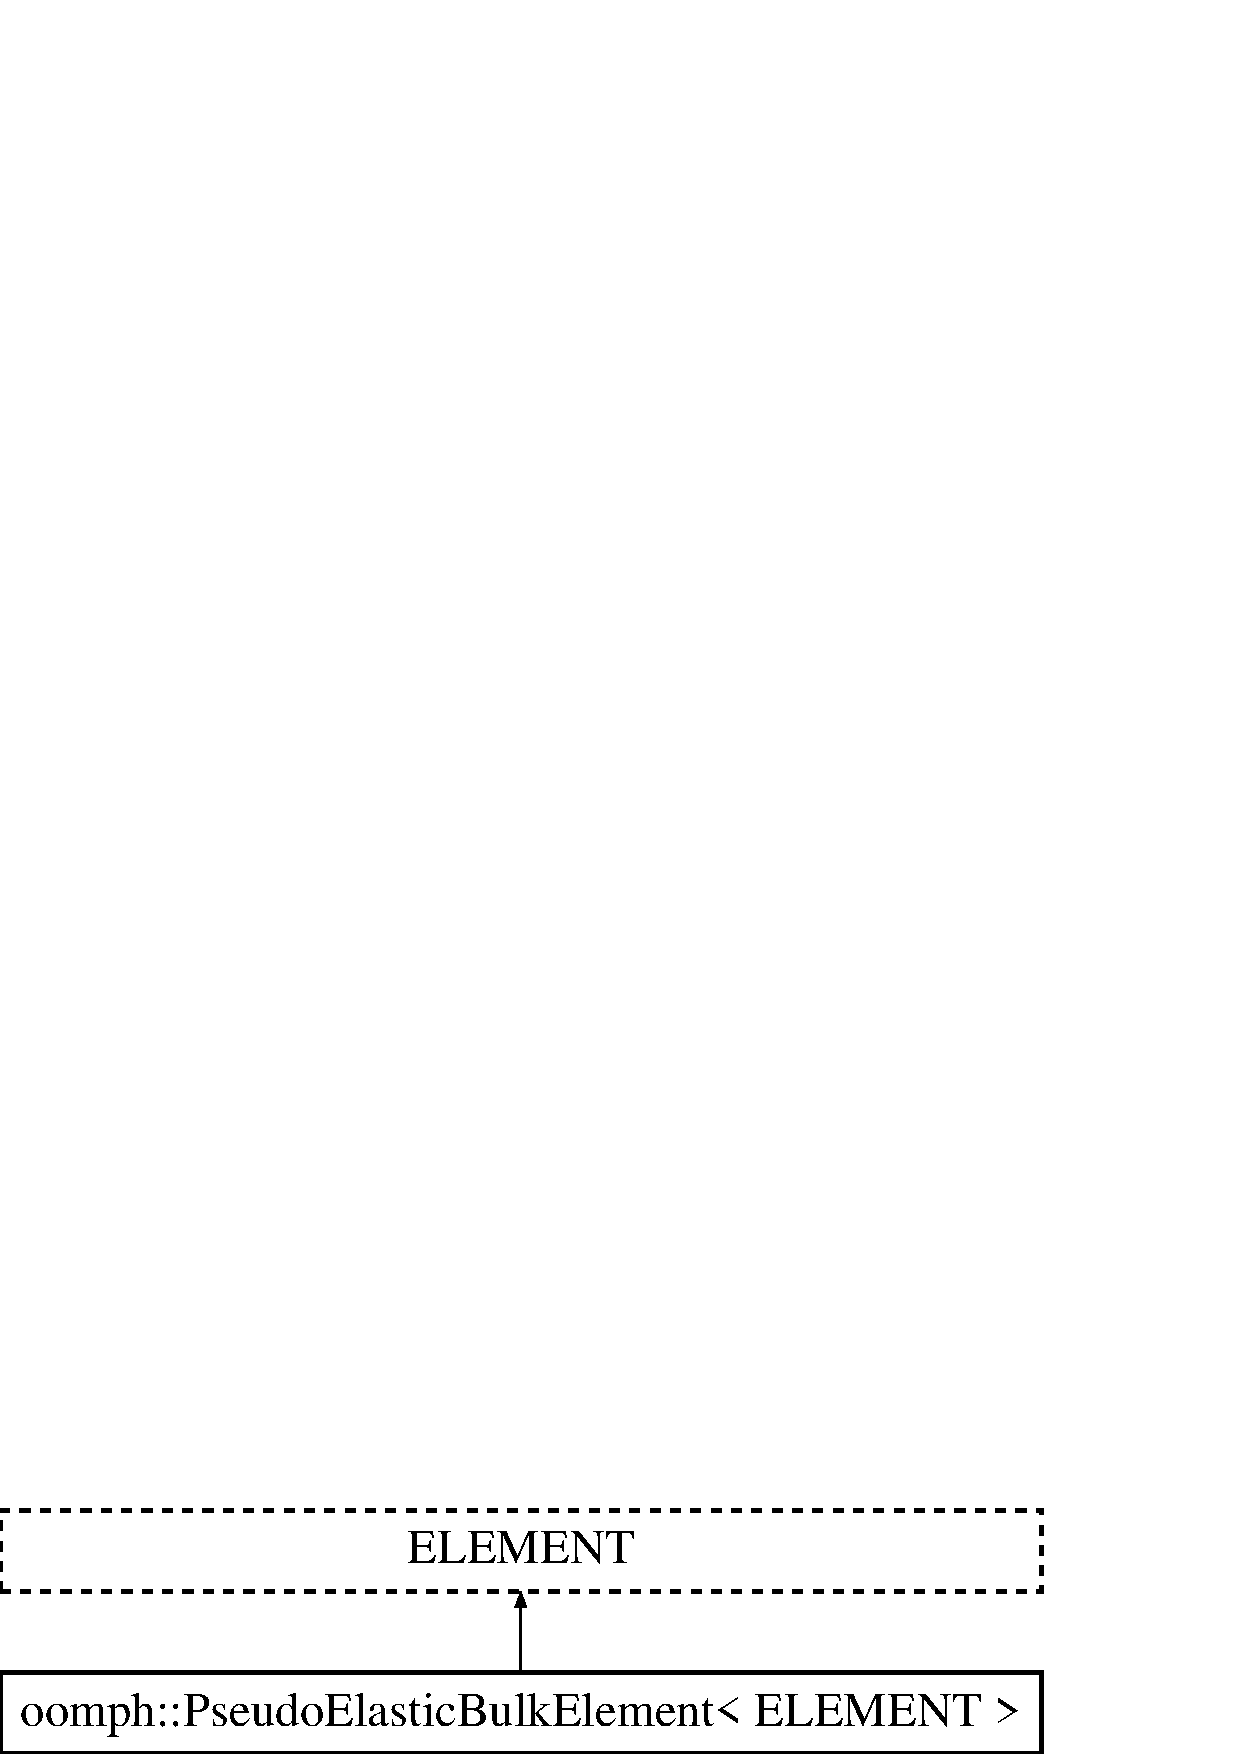
\includegraphics[height=2.000000cm]{classoomph_1_1PseudoElasticBulkElement}
\end{center}
\end{figure}
\subsection*{Public Member Functions}
\begin{DoxyCompactItemize}
\item 
\hyperlink{classoomph_1_1PseudoElasticBulkElement_a38c03edd9639522e713ef9bf679d7e5a}{Pseudo\+Elastic\+Bulk\+Element} ()
\begin{DoxyCompactList}\small\item\em Constructor. \end{DoxyCompactList}\item 
unsigned \hyperlink{classoomph_1_1PseudoElasticBulkElement_a18674d52b96db8800d31e89ffd465175}{ndof\+\_\+types} () const
\begin{DoxyCompactList}\small\item\em Returns the number of D\+OF types associated with this element\+: Twice the number of spatial dimensions (for the constrained and unconstrained nodal positions). \end{DoxyCompactList}\item 
void \hyperlink{classoomph_1_1PseudoElasticBulkElement_a8f1dc2011100324953293470a18f3080}{get\+\_\+dof\+\_\+numbers\+\_\+for\+\_\+unknowns} (std\+::list$<$ std\+::pair$<$ unsigned long, unsigned $>$ $>$ \&dof\+\_\+lookup\+\_\+list) const
\begin{DoxyCompactList}\small\item\em Create a list of pairs for all unknowns in this element, so that the first entry in each pair contains the global equation number of the unknown, while the second one contains the number of the \char`\"{}\+D\+O\+F\char`\"{} that this unknown is associated with. (Function can obviously only be called if the equation numbering scheme has been set up.)~\newline
E.\+g. in a 3D problem there are 6 types of D\+OF\+:~\newline
0 -\/ x displacement (without lagr mult traction)~\newline
1 -\/ y displacement (without lagr mult traction)~\newline
2 -\/ z displacement (without lagr mult traction)~\newline
4 -\/ x displacement (with lagr mult traction)~\newline
5 -\/ y displacement (with lagr mult traction)~\newline
6 -\/ z displacement (with lagr mult traction)~\newline
. \end{DoxyCompactList}\end{DoxyCompactItemize}


\subsection{Detailed Description}
\subsubsection*{template$<$class E\+L\+E\+M\+E\+NT$>$\newline
class oomph\+::\+Pseudo\+Elastic\+Bulk\+Element$<$ E\+L\+E\+M\+E\+N\+T $>$}

Pseudo-\/\+Elastic Solid element class to overload the block preconditioner methods \hyperlink{classoomph_1_1PseudoElasticBulkElement_a18674d52b96db8800d31e89ffd465175}{ndof\+\_\+types()} and \hyperlink{classoomph_1_1PseudoElasticBulkElement_a8f1dc2011100324953293470a18f3080}{get\+\_\+dof\+\_\+numbers\+\_\+for\+\_\+unknowns()} to differentiate between D\+O\+Fs subject to Lagrange multiplier and those that are not. 

Definition at line 58 of file prescribed\+\_\+displ\+\_\+lagr\+\_\+mult\+\_\+precond.\+cc.



\subsection{Constructor \& Destructor Documentation}
\mbox{\Hypertarget{classoomph_1_1PseudoElasticBulkElement_a38c03edd9639522e713ef9bf679d7e5a}\label{classoomph_1_1PseudoElasticBulkElement_a38c03edd9639522e713ef9bf679d7e5a}} 
\index{oomph\+::\+Pseudo\+Elastic\+Bulk\+Element@{oomph\+::\+Pseudo\+Elastic\+Bulk\+Element}!Pseudo\+Elastic\+Bulk\+Element@{Pseudo\+Elastic\+Bulk\+Element}}
\index{Pseudo\+Elastic\+Bulk\+Element@{Pseudo\+Elastic\+Bulk\+Element}!oomph\+::\+Pseudo\+Elastic\+Bulk\+Element@{oomph\+::\+Pseudo\+Elastic\+Bulk\+Element}}
\subsubsection{\texorpdfstring{Pseudo\+Elastic\+Bulk\+Element()}{PseudoElasticBulkElement()}}
{\footnotesize\ttfamily template$<$class E\+L\+E\+M\+E\+NT $>$ \\
\hyperlink{classoomph_1_1PseudoElasticBulkElement}{oomph\+::\+Pseudo\+Elastic\+Bulk\+Element}$<$ E\+L\+E\+M\+E\+NT $>$\+::\hyperlink{classoomph_1_1PseudoElasticBulkElement}{Pseudo\+Elastic\+Bulk\+Element} (\begin{DoxyParamCaption}{ }\end{DoxyParamCaption})\hspace{0.3cm}{\ttfamily [inline]}}



Constructor. 



Definition at line 65 of file prescribed\+\_\+displ\+\_\+lagr\+\_\+mult\+\_\+precond.\+cc.



\subsection{Member Function Documentation}
\mbox{\Hypertarget{classoomph_1_1PseudoElasticBulkElement_a8f1dc2011100324953293470a18f3080}\label{classoomph_1_1PseudoElasticBulkElement_a8f1dc2011100324953293470a18f3080}} 
\index{oomph\+::\+Pseudo\+Elastic\+Bulk\+Element@{oomph\+::\+Pseudo\+Elastic\+Bulk\+Element}!get\+\_\+dof\+\_\+numbers\+\_\+for\+\_\+unknowns@{get\+\_\+dof\+\_\+numbers\+\_\+for\+\_\+unknowns}}
\index{get\+\_\+dof\+\_\+numbers\+\_\+for\+\_\+unknowns@{get\+\_\+dof\+\_\+numbers\+\_\+for\+\_\+unknowns}!oomph\+::\+Pseudo\+Elastic\+Bulk\+Element@{oomph\+::\+Pseudo\+Elastic\+Bulk\+Element}}
\subsubsection{\texorpdfstring{get\+\_\+dof\+\_\+numbers\+\_\+for\+\_\+unknowns()}{get\_dof\_numbers\_for\_unknowns()}}
{\footnotesize\ttfamily template$<$class E\+L\+E\+M\+E\+NT $>$ \\
void \hyperlink{classoomph_1_1PseudoElasticBulkElement}{oomph\+::\+Pseudo\+Elastic\+Bulk\+Element}$<$ E\+L\+E\+M\+E\+NT $>$\+::get\+\_\+dof\+\_\+numbers\+\_\+for\+\_\+unknowns (\begin{DoxyParamCaption}\item[{std\+::list$<$ std\+::pair$<$ unsigned long, unsigned $>$ $>$ \&}]{dof\+\_\+lookup\+\_\+list }\end{DoxyParamCaption}) const\hspace{0.3cm}{\ttfamily [inline]}}



Create a list of pairs for all unknowns in this element, so that the first entry in each pair contains the global equation number of the unknown, while the second one contains the number of the \char`\"{}\+D\+O\+F\char`\"{} that this unknown is associated with. (Function can obviously only be called if the equation numbering scheme has been set up.)~\newline
E.\+g. in a 3D problem there are 6 types of D\+OF\+:~\newline
0 -\/ x displacement (without lagr mult traction)~\newline
1 -\/ y displacement (without lagr mult traction)~\newline
2 -\/ z displacement (without lagr mult traction)~\newline
4 -\/ x displacement (with lagr mult traction)~\newline
5 -\/ y displacement (with lagr mult traction)~\newline
6 -\/ z displacement (with lagr mult traction)~\newline
. 



Definition at line 88 of file prescribed\+\_\+displ\+\_\+lagr\+\_\+mult\+\_\+precond.\+cc.

\mbox{\Hypertarget{classoomph_1_1PseudoElasticBulkElement_a18674d52b96db8800d31e89ffd465175}\label{classoomph_1_1PseudoElasticBulkElement_a18674d52b96db8800d31e89ffd465175}} 
\index{oomph\+::\+Pseudo\+Elastic\+Bulk\+Element@{oomph\+::\+Pseudo\+Elastic\+Bulk\+Element}!ndof\+\_\+types@{ndof\+\_\+types}}
\index{ndof\+\_\+types@{ndof\+\_\+types}!oomph\+::\+Pseudo\+Elastic\+Bulk\+Element@{oomph\+::\+Pseudo\+Elastic\+Bulk\+Element}}
\subsubsection{\texorpdfstring{ndof\+\_\+types()}{ndof\_types()}}
{\footnotesize\ttfamily template$<$class E\+L\+E\+M\+E\+NT $>$ \\
unsigned \hyperlink{classoomph_1_1PseudoElasticBulkElement}{oomph\+::\+Pseudo\+Elastic\+Bulk\+Element}$<$ E\+L\+E\+M\+E\+NT $>$\+::ndof\+\_\+types (\begin{DoxyParamCaption}{ }\end{DoxyParamCaption}) const\hspace{0.3cm}{\ttfamily [inline]}}



Returns the number of D\+OF types associated with this element\+: Twice the number of spatial dimensions (for the constrained and unconstrained nodal positions). 



Definition at line 70 of file prescribed\+\_\+displ\+\_\+lagr\+\_\+mult\+\_\+precond.\+cc.



The documentation for this class was generated from the following file\+:\begin{DoxyCompactItemize}
\item 
\hyperlink{prescribed__displ__lagr__mult__precond_8cc}{prescribed\+\_\+displ\+\_\+lagr\+\_\+mult\+\_\+precond.\+cc}\end{DoxyCompactItemize}

\hypertarget{classWarpedLine}{}\section{Warped\+Line Class Reference}
\label{classWarpedLine}\index{Warped\+Line@{Warped\+Line}}


Warped line in 2D space.  


Inheritance diagram for Warped\+Line\+:\begin{figure}[H]
\begin{center}
\leavevmode
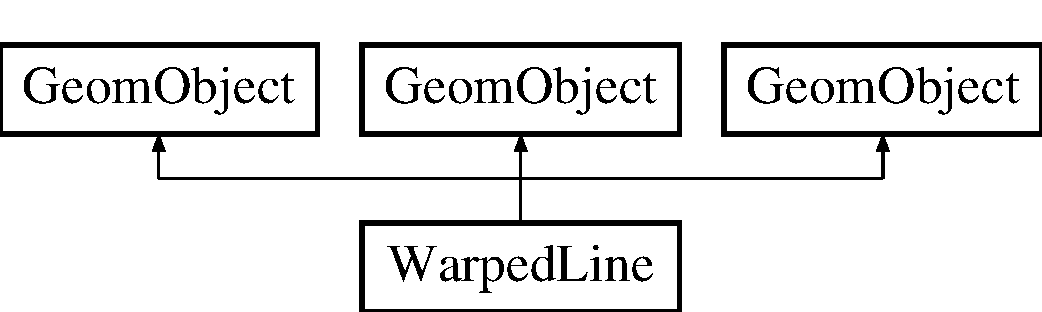
\includegraphics[height=2.000000cm]{classWarpedLine}
\end{center}
\end{figure}
\subsection*{Public Member Functions}
\begin{DoxyCompactItemize}
\item 
\hyperlink{classWarpedLine_a9d80dca2c907b426f7130579c94f3310}{Warped\+Line} (const double \&\hyperlink{classWarpedLine_ae43c2f997b9c0de62783375341ac5794}{ampl})
\begin{DoxyCompactList}\small\item\em Constructor\+: Specify amplitude of deflection from straight horizontal line. \end{DoxyCompactList}\item 
\hyperlink{classWarpedLine_a53a7426303864ea2d34aeba0a3f6324f}{Warped\+Line} (const \hyperlink{classWarpedLine}{Warped\+Line} \&dummy)
\begin{DoxyCompactList}\small\item\em Broken copy constructor. \end{DoxyCompactList}\item 
void \hyperlink{classWarpedLine_ae2ee796906c0caa7e94f277f6fc499e1}{operator=} (const \hyperlink{classWarpedLine}{Warped\+Line} \&)
\begin{DoxyCompactList}\small\item\em Broken assignment operator. \end{DoxyCompactList}\item 
\hyperlink{classWarpedLine_a4cb07fb7f06d42e2008afe65d8750cad}{$\sim$\+Warped\+Line} ()
\begin{DoxyCompactList}\small\item\em Empty Destructor. \end{DoxyCompactList}\item 
void \hyperlink{classWarpedLine_aaeef89818148ee3a305c561e91c8851d}{position} (const Vector$<$ double $>$ \&zeta, Vector$<$ double $>$ \&r) const
\begin{DoxyCompactList}\small\item\em Position vector at Lagrangian coordinate zeta. \end{DoxyCompactList}\item 
void \hyperlink{classWarpedLine_a415d50f6bb49bd903015b51c66e93cd2}{position} (const unsigned \&t, const Vector$<$ double $>$ \&zeta, Vector$<$ double $>$ \&r) const
\begin{DoxyCompactList}\small\item\em Parametrised position on object\+: r(zeta). Evaluated at previous timestep. t=0\+: current time; t$>$0\+: previous timestep. Forward to steady version. \end{DoxyCompactList}\item 
double \& \hyperlink{classWarpedLine_ae43c2f997b9c0de62783375341ac5794}{ampl} ()
\begin{DoxyCompactList}\small\item\em Access to amplitude. \end{DoxyCompactList}\item 
unsigned \hyperlink{classWarpedLine_aa4157cd4ff2e80f33b106b7ed4e4d804}{ngeom\+\_\+data} () const
\begin{DoxyCompactList}\small\item\em How many items of Data does the shape of the object depend on? None. \end{DoxyCompactList}\item 
\hyperlink{classWarpedLine_a9d80dca2c907b426f7130579c94f3310}{Warped\+Line} (const double \&\hyperlink{classWarpedLine_ae43c2f997b9c0de62783375341ac5794}{ampl})
\begin{DoxyCompactList}\small\item\em Constructor\+: Specify amplitude of deflection from straight horizontal line. \end{DoxyCompactList}\item 
\hyperlink{classWarpedLine_a53a7426303864ea2d34aeba0a3f6324f}{Warped\+Line} (const \hyperlink{classWarpedLine}{Warped\+Line} \&dummy)
\begin{DoxyCompactList}\small\item\em Broken copy constructor. \end{DoxyCompactList}\item 
void \hyperlink{classWarpedLine_ae2ee796906c0caa7e94f277f6fc499e1}{operator=} (const \hyperlink{classWarpedLine}{Warped\+Line} \&)
\begin{DoxyCompactList}\small\item\em Broken assignment operator. \end{DoxyCompactList}\item 
\hyperlink{classWarpedLine_a4cb07fb7f06d42e2008afe65d8750cad}{$\sim$\+Warped\+Line} ()
\begin{DoxyCompactList}\small\item\em Empty Destructor. \end{DoxyCompactList}\item 
void \hyperlink{classWarpedLine_aaeef89818148ee3a305c561e91c8851d}{position} (const Vector$<$ double $>$ \&zeta, Vector$<$ double $>$ \&r) const
\begin{DoxyCompactList}\small\item\em Position vector at Lagrangian coordinate zeta. \end{DoxyCompactList}\item 
void \hyperlink{classWarpedLine_a415d50f6bb49bd903015b51c66e93cd2}{position} (const unsigned \&t, const Vector$<$ double $>$ \&zeta, Vector$<$ double $>$ \&r) const
\begin{DoxyCompactList}\small\item\em Parametrised position on object\+: r(zeta). Evaluated at previous timestep. t=0\+: current time; t$>$0\+: previous timestep. Forward to steady version. \end{DoxyCompactList}\item 
double \& \hyperlink{classWarpedLine_ae43c2f997b9c0de62783375341ac5794}{ampl} ()
\begin{DoxyCompactList}\small\item\em Access to amplitude. \end{DoxyCompactList}\item 
\hyperlink{classWarpedLine_a9d80dca2c907b426f7130579c94f3310}{Warped\+Line} (const double \&\hyperlink{classWarpedLine_ae43c2f997b9c0de62783375341ac5794}{ampl})
\begin{DoxyCompactList}\small\item\em Constructor\+: Specify amplitude of deflection from straight horizontal line. \end{DoxyCompactList}\item 
\hyperlink{classWarpedLine_a53a7426303864ea2d34aeba0a3f6324f}{Warped\+Line} (const \hyperlink{classWarpedLine}{Warped\+Line} \&dummy)
\begin{DoxyCompactList}\small\item\em Broken copy constructor. \end{DoxyCompactList}\item 
void \hyperlink{classWarpedLine_ae2ee796906c0caa7e94f277f6fc499e1}{operator=} (const \hyperlink{classWarpedLine}{Warped\+Line} \&)
\begin{DoxyCompactList}\small\item\em Broken assignment operator. \end{DoxyCompactList}\item 
\hyperlink{classWarpedLine_a4cb07fb7f06d42e2008afe65d8750cad}{$\sim$\+Warped\+Line} ()
\begin{DoxyCompactList}\small\item\em Empty Destructor. \end{DoxyCompactList}\item 
void \hyperlink{classWarpedLine_aaeef89818148ee3a305c561e91c8851d}{position} (const Vector$<$ double $>$ \&zeta, Vector$<$ double $>$ \&r) const
\begin{DoxyCompactList}\small\item\em Position vector at Lagrangian coordinate zeta. \end{DoxyCompactList}\item 
void \hyperlink{classWarpedLine_a415d50f6bb49bd903015b51c66e93cd2}{position} (const unsigned \&t, const Vector$<$ double $>$ \&zeta, Vector$<$ double $>$ \&r) const
\begin{DoxyCompactList}\small\item\em Parametrised position on object\+: r(zeta). Evaluated at previous timestep. t=0\+: current time; t$>$0\+: previous timestep. Forward to steady version. \end{DoxyCompactList}\item 
double \& \hyperlink{classWarpedLine_ae43c2f997b9c0de62783375341ac5794}{ampl} ()
\begin{DoxyCompactList}\small\item\em Access to amplitude. \end{DoxyCompactList}\item 
unsigned \hyperlink{classWarpedLine_aa4157cd4ff2e80f33b106b7ed4e4d804}{ngeom\+\_\+data} () const
\begin{DoxyCompactList}\small\item\em How many items of Data does the shape of the object depend on? None. \end{DoxyCompactList}\end{DoxyCompactItemize}
\subsection*{Private Attributes}
\begin{DoxyCompactItemize}
\item 
double \hyperlink{classWarpedLine_ac44286e84ff213e67e0f247d00ad50af}{Ampl}
\begin{DoxyCompactList}\small\item\em Amplitude of perturbation. \end{DoxyCompactList}\end{DoxyCompactItemize}


\subsection{Detailed Description}
Warped line in 2D space. 

Definition at line 70 of file prescribed\+\_\+displ\+\_\+lagr\+\_\+mult.\+cc.



\subsection{Constructor \& Destructor Documentation}
\mbox{\Hypertarget{classWarpedLine_a9d80dca2c907b426f7130579c94f3310}\label{classWarpedLine_a9d80dca2c907b426f7130579c94f3310}} 
\index{Warped\+Line@{Warped\+Line}!Warped\+Line@{Warped\+Line}}
\index{Warped\+Line@{Warped\+Line}!Warped\+Line@{Warped\+Line}}
\subsubsection{\texorpdfstring{Warped\+Line()}{WarpedLine()}\hspace{0.1cm}{\footnotesize\ttfamily [1/6]}}
{\footnotesize\ttfamily Warped\+Line\+::\+Warped\+Line (\begin{DoxyParamCaption}\item[{const double \&}]{ampl }\end{DoxyParamCaption})\hspace{0.3cm}{\ttfamily [inline]}}



Constructor\+: Specify amplitude of deflection from straight horizontal line. 



Definition at line 76 of file prescribed\+\_\+displ\+\_\+lagr\+\_\+mult.\+cc.

\mbox{\Hypertarget{classWarpedLine_a53a7426303864ea2d34aeba0a3f6324f}\label{classWarpedLine_a53a7426303864ea2d34aeba0a3f6324f}} 
\index{Warped\+Line@{Warped\+Line}!Warped\+Line@{Warped\+Line}}
\index{Warped\+Line@{Warped\+Line}!Warped\+Line@{Warped\+Line}}
\subsubsection{\texorpdfstring{Warped\+Line()}{WarpedLine()}\hspace{0.1cm}{\footnotesize\ttfamily [2/6]}}
{\footnotesize\ttfamily Warped\+Line\+::\+Warped\+Line (\begin{DoxyParamCaption}\item[{const \hyperlink{classWarpedLine}{Warped\+Line} \&}]{dummy }\end{DoxyParamCaption})\hspace{0.3cm}{\ttfamily [inline]}}



Broken copy constructor. 



Definition at line 82 of file prescribed\+\_\+displ\+\_\+lagr\+\_\+mult.\+cc.

\mbox{\Hypertarget{classWarpedLine_a4cb07fb7f06d42e2008afe65d8750cad}\label{classWarpedLine_a4cb07fb7f06d42e2008afe65d8750cad}} 
\index{Warped\+Line@{Warped\+Line}!````~Warped\+Line@{$\sim$\+Warped\+Line}}
\index{````~Warped\+Line@{$\sim$\+Warped\+Line}!Warped\+Line@{Warped\+Line}}
\subsubsection{\texorpdfstring{$\sim$\+Warped\+Line()}{~WarpedLine()}\hspace{0.1cm}{\footnotesize\ttfamily [1/3]}}
{\footnotesize\ttfamily Warped\+Line\+::$\sim$\+Warped\+Line (\begin{DoxyParamCaption}{ }\end{DoxyParamCaption})\hspace{0.3cm}{\ttfamily [inline]}}



Empty Destructor. 



Definition at line 95 of file prescribed\+\_\+displ\+\_\+lagr\+\_\+mult.\+cc.

\mbox{\Hypertarget{classWarpedLine_a9d80dca2c907b426f7130579c94f3310}\label{classWarpedLine_a9d80dca2c907b426f7130579c94f3310}} 
\index{Warped\+Line@{Warped\+Line}!Warped\+Line@{Warped\+Line}}
\index{Warped\+Line@{Warped\+Line}!Warped\+Line@{Warped\+Line}}
\subsubsection{\texorpdfstring{Warped\+Line()}{WarpedLine()}\hspace{0.1cm}{\footnotesize\ttfamily [3/6]}}
{\footnotesize\ttfamily Warped\+Line\+::\+Warped\+Line (\begin{DoxyParamCaption}\item[{const double \&}]{ampl }\end{DoxyParamCaption})\hspace{0.3cm}{\ttfamily [inline]}}



Constructor\+: Specify amplitude of deflection from straight horizontal line. 



Definition at line 55 of file prescribed\+\_\+displ\+\_\+lagr\+\_\+mult2.\+cc.

\mbox{\Hypertarget{classWarpedLine_a53a7426303864ea2d34aeba0a3f6324f}\label{classWarpedLine_a53a7426303864ea2d34aeba0a3f6324f}} 
\index{Warped\+Line@{Warped\+Line}!Warped\+Line@{Warped\+Line}}
\index{Warped\+Line@{Warped\+Line}!Warped\+Line@{Warped\+Line}}
\subsubsection{\texorpdfstring{Warped\+Line()}{WarpedLine()}\hspace{0.1cm}{\footnotesize\ttfamily [4/6]}}
{\footnotesize\ttfamily Warped\+Line\+::\+Warped\+Line (\begin{DoxyParamCaption}\item[{const \hyperlink{classWarpedLine}{Warped\+Line} \&}]{dummy }\end{DoxyParamCaption})\hspace{0.3cm}{\ttfamily [inline]}}



Broken copy constructor. 



Definition at line 61 of file prescribed\+\_\+displ\+\_\+lagr\+\_\+mult2.\+cc.

\mbox{\Hypertarget{classWarpedLine_a4cb07fb7f06d42e2008afe65d8750cad}\label{classWarpedLine_a4cb07fb7f06d42e2008afe65d8750cad}} 
\index{Warped\+Line@{Warped\+Line}!````~Warped\+Line@{$\sim$\+Warped\+Line}}
\index{````~Warped\+Line@{$\sim$\+Warped\+Line}!Warped\+Line@{Warped\+Line}}
\subsubsection{\texorpdfstring{$\sim$\+Warped\+Line()}{~WarpedLine()}\hspace{0.1cm}{\footnotesize\ttfamily [2/3]}}
{\footnotesize\ttfamily Warped\+Line\+::$\sim$\+Warped\+Line (\begin{DoxyParamCaption}{ }\end{DoxyParamCaption})\hspace{0.3cm}{\ttfamily [inline]}}



Empty Destructor. 



Definition at line 74 of file prescribed\+\_\+displ\+\_\+lagr\+\_\+mult2.\+cc.

\mbox{\Hypertarget{classWarpedLine_a9d80dca2c907b426f7130579c94f3310}\label{classWarpedLine_a9d80dca2c907b426f7130579c94f3310}} 
\index{Warped\+Line@{Warped\+Line}!Warped\+Line@{Warped\+Line}}
\index{Warped\+Line@{Warped\+Line}!Warped\+Line@{Warped\+Line}}
\subsubsection{\texorpdfstring{Warped\+Line()}{WarpedLine()}\hspace{0.1cm}{\footnotesize\ttfamily [5/6]}}
{\footnotesize\ttfamily Warped\+Line\+::\+Warped\+Line (\begin{DoxyParamCaption}\item[{const double \&}]{ampl }\end{DoxyParamCaption})\hspace{0.3cm}{\ttfamily [inline]}}



Constructor\+: Specify amplitude of deflection from straight horizontal line. 



Definition at line 223 of file prescribed\+\_\+displ\+\_\+lagr\+\_\+mult\+\_\+precond.\+cc.

\mbox{\Hypertarget{classWarpedLine_a53a7426303864ea2d34aeba0a3f6324f}\label{classWarpedLine_a53a7426303864ea2d34aeba0a3f6324f}} 
\index{Warped\+Line@{Warped\+Line}!Warped\+Line@{Warped\+Line}}
\index{Warped\+Line@{Warped\+Line}!Warped\+Line@{Warped\+Line}}
\subsubsection{\texorpdfstring{Warped\+Line()}{WarpedLine()}\hspace{0.1cm}{\footnotesize\ttfamily [6/6]}}
{\footnotesize\ttfamily Warped\+Line\+::\+Warped\+Line (\begin{DoxyParamCaption}\item[{const \hyperlink{classWarpedLine}{Warped\+Line} \&}]{dummy }\end{DoxyParamCaption})\hspace{0.3cm}{\ttfamily [inline]}}



Broken copy constructor. 



Definition at line 229 of file prescribed\+\_\+displ\+\_\+lagr\+\_\+mult\+\_\+precond.\+cc.

\mbox{\Hypertarget{classWarpedLine_a4cb07fb7f06d42e2008afe65d8750cad}\label{classWarpedLine_a4cb07fb7f06d42e2008afe65d8750cad}} 
\index{Warped\+Line@{Warped\+Line}!````~Warped\+Line@{$\sim$\+Warped\+Line}}
\index{````~Warped\+Line@{$\sim$\+Warped\+Line}!Warped\+Line@{Warped\+Line}}
\subsubsection{\texorpdfstring{$\sim$\+Warped\+Line()}{~WarpedLine()}\hspace{0.1cm}{\footnotesize\ttfamily [3/3]}}
{\footnotesize\ttfamily Warped\+Line\+::$\sim$\+Warped\+Line (\begin{DoxyParamCaption}{ }\end{DoxyParamCaption})\hspace{0.3cm}{\ttfamily [inline]}}



Empty Destructor. 



Definition at line 242 of file prescribed\+\_\+displ\+\_\+lagr\+\_\+mult\+\_\+precond.\+cc.



\subsection{Member Function Documentation}
\mbox{\Hypertarget{classWarpedLine_ae43c2f997b9c0de62783375341ac5794}\label{classWarpedLine_ae43c2f997b9c0de62783375341ac5794}} 
\index{Warped\+Line@{Warped\+Line}!ampl@{ampl}}
\index{ampl@{ampl}!Warped\+Line@{Warped\+Line}}
\subsubsection{\texorpdfstring{ampl()}{ampl()}\hspace{0.1cm}{\footnotesize\ttfamily [1/3]}}
{\footnotesize\ttfamily double\& Warped\+Line\+::ampl (\begin{DoxyParamCaption}{ }\end{DoxyParamCaption})\hspace{0.3cm}{\ttfamily [inline]}}



Access to amplitude. 



Definition at line 94 of file prescribed\+\_\+displ\+\_\+lagr\+\_\+mult2.\+cc.



References Global\+\_\+\+Physical\+\_\+\+Variables\+::\+Boundary\+\_\+geom\+\_\+object(), and Global\+\_\+\+Physical\+\_\+\+Variables\+::\+Nu.

\mbox{\Hypertarget{classWarpedLine_ae43c2f997b9c0de62783375341ac5794}\label{classWarpedLine_ae43c2f997b9c0de62783375341ac5794}} 
\index{Warped\+Line@{Warped\+Line}!ampl@{ampl}}
\index{ampl@{ampl}!Warped\+Line@{Warped\+Line}}
\subsubsection{\texorpdfstring{ampl()}{ampl()}\hspace{0.1cm}{\footnotesize\ttfamily [2/3]}}
{\footnotesize\ttfamily double\& Warped\+Line\+::ampl (\begin{DoxyParamCaption}{ }\end{DoxyParamCaption})\hspace{0.3cm}{\ttfamily [inline]}}



Access to amplitude. 



Definition at line 115 of file prescribed\+\_\+displ\+\_\+lagr\+\_\+mult.\+cc.



Referenced by main().

\mbox{\Hypertarget{classWarpedLine_ae43c2f997b9c0de62783375341ac5794}\label{classWarpedLine_ae43c2f997b9c0de62783375341ac5794}} 
\index{Warped\+Line@{Warped\+Line}!ampl@{ampl}}
\index{ampl@{ampl}!Warped\+Line@{Warped\+Line}}
\subsubsection{\texorpdfstring{ampl()}{ampl()}\hspace{0.1cm}{\footnotesize\ttfamily [3/3]}}
{\footnotesize\ttfamily double\& Warped\+Line\+::ampl (\begin{DoxyParamCaption}{ }\end{DoxyParamCaption})\hspace{0.3cm}{\ttfamily [inline]}}



Access to amplitude. 



Definition at line 262 of file prescribed\+\_\+displ\+\_\+lagr\+\_\+mult\+\_\+precond.\+cc.

\mbox{\Hypertarget{classWarpedLine_aa4157cd4ff2e80f33b106b7ed4e4d804}\label{classWarpedLine_aa4157cd4ff2e80f33b106b7ed4e4d804}} 
\index{Warped\+Line@{Warped\+Line}!ngeom\+\_\+data@{ngeom\+\_\+data}}
\index{ngeom\+\_\+data@{ngeom\+\_\+data}!Warped\+Line@{Warped\+Line}}
\subsubsection{\texorpdfstring{ngeom\+\_\+data()}{ngeom\_data()}\hspace{0.1cm}{\footnotesize\ttfamily [1/2]}}
{\footnotesize\ttfamily unsigned Warped\+Line\+::ngeom\+\_\+data (\begin{DoxyParamCaption}{ }\end{DoxyParamCaption}) const\hspace{0.3cm}{\ttfamily [inline]}}



How many items of Data does the shape of the object depend on? None. 



Definition at line 119 of file prescribed\+\_\+displ\+\_\+lagr\+\_\+mult.\+cc.

\mbox{\Hypertarget{classWarpedLine_aa4157cd4ff2e80f33b106b7ed4e4d804}\label{classWarpedLine_aa4157cd4ff2e80f33b106b7ed4e4d804}} 
\index{Warped\+Line@{Warped\+Line}!ngeom\+\_\+data@{ngeom\+\_\+data}}
\index{ngeom\+\_\+data@{ngeom\+\_\+data}!Warped\+Line@{Warped\+Line}}
\subsubsection{\texorpdfstring{ngeom\+\_\+data()}{ngeom\_data()}\hspace{0.1cm}{\footnotesize\ttfamily [2/2]}}
{\footnotesize\ttfamily unsigned Warped\+Line\+::ngeom\+\_\+data (\begin{DoxyParamCaption}{ }\end{DoxyParamCaption}) const\hspace{0.3cm}{\ttfamily [inline]}}



How many items of Data does the shape of the object depend on? None. 



Definition at line 266 of file prescribed\+\_\+displ\+\_\+lagr\+\_\+mult\+\_\+precond.\+cc.



References Global\+\_\+\+Physical\+\_\+\+Variables\+::\+Boundary\+\_\+geom\+\_\+object, and Global\+\_\+\+Physical\+\_\+\+Variables\+::\+Nu.

\mbox{\Hypertarget{classWarpedLine_ae2ee796906c0caa7e94f277f6fc499e1}\label{classWarpedLine_ae2ee796906c0caa7e94f277f6fc499e1}} 
\index{Warped\+Line@{Warped\+Line}!operator=@{operator=}}
\index{operator=@{operator=}!Warped\+Line@{Warped\+Line}}
\subsubsection{\texorpdfstring{operator=()}{operator=()}\hspace{0.1cm}{\footnotesize\ttfamily [1/3]}}
{\footnotesize\ttfamily void Warped\+Line\+::operator= (\begin{DoxyParamCaption}\item[{const \hyperlink{classWarpedLine}{Warped\+Line} \&}]{ }\end{DoxyParamCaption})\hspace{0.3cm}{\ttfamily [inline]}}



Broken assignment operator. 



Definition at line 67 of file prescribed\+\_\+displ\+\_\+lagr\+\_\+mult2.\+cc.

\mbox{\Hypertarget{classWarpedLine_ae2ee796906c0caa7e94f277f6fc499e1}\label{classWarpedLine_ae2ee796906c0caa7e94f277f6fc499e1}} 
\index{Warped\+Line@{Warped\+Line}!operator=@{operator=}}
\index{operator=@{operator=}!Warped\+Line@{Warped\+Line}}
\subsubsection{\texorpdfstring{operator=()}{operator=()}\hspace{0.1cm}{\footnotesize\ttfamily [2/3]}}
{\footnotesize\ttfamily void Warped\+Line\+::operator= (\begin{DoxyParamCaption}\item[{const \hyperlink{classWarpedLine}{Warped\+Line} \&}]{ }\end{DoxyParamCaption})\hspace{0.3cm}{\ttfamily [inline]}}



Broken assignment operator. 



Definition at line 88 of file prescribed\+\_\+displ\+\_\+lagr\+\_\+mult.\+cc.

\mbox{\Hypertarget{classWarpedLine_ae2ee796906c0caa7e94f277f6fc499e1}\label{classWarpedLine_ae2ee796906c0caa7e94f277f6fc499e1}} 
\index{Warped\+Line@{Warped\+Line}!operator=@{operator=}}
\index{operator=@{operator=}!Warped\+Line@{Warped\+Line}}
\subsubsection{\texorpdfstring{operator=()}{operator=()}\hspace{0.1cm}{\footnotesize\ttfamily [3/3]}}
{\footnotesize\ttfamily void Warped\+Line\+::operator= (\begin{DoxyParamCaption}\item[{const \hyperlink{classWarpedLine}{Warped\+Line} \&}]{ }\end{DoxyParamCaption})\hspace{0.3cm}{\ttfamily [inline]}}



Broken assignment operator. 



Definition at line 235 of file prescribed\+\_\+displ\+\_\+lagr\+\_\+mult\+\_\+precond.\+cc.

\mbox{\Hypertarget{classWarpedLine_aaeef89818148ee3a305c561e91c8851d}\label{classWarpedLine_aaeef89818148ee3a305c561e91c8851d}} 
\index{Warped\+Line@{Warped\+Line}!position@{position}}
\index{position@{position}!Warped\+Line@{Warped\+Line}}
\subsubsection{\texorpdfstring{position()}{position()}\hspace{0.1cm}{\footnotesize\ttfamily [1/6]}}
{\footnotesize\ttfamily void Warped\+Line\+::position (\begin{DoxyParamCaption}\item[{const Vector$<$ double $>$ \&}]{zeta,  }\item[{Vector$<$ double $>$ \&}]{r }\end{DoxyParamCaption}) const\hspace{0.3cm}{\ttfamily [inline]}}



Position vector at Lagrangian coordinate zeta. 



Definition at line 77 of file prescribed\+\_\+displ\+\_\+lagr\+\_\+mult2.\+cc.

\mbox{\Hypertarget{classWarpedLine_a415d50f6bb49bd903015b51c66e93cd2}\label{classWarpedLine_a415d50f6bb49bd903015b51c66e93cd2}} 
\index{Warped\+Line@{Warped\+Line}!position@{position}}
\index{position@{position}!Warped\+Line@{Warped\+Line}}
\subsubsection{\texorpdfstring{position()}{position()}\hspace{0.1cm}{\footnotesize\ttfamily [2/6]}}
{\footnotesize\ttfamily void Warped\+Line\+::position (\begin{DoxyParamCaption}\item[{const unsigned \&}]{t,  }\item[{const Vector$<$ double $>$ \&}]{zeta,  }\item[{Vector$<$ double $>$ \&}]{r }\end{DoxyParamCaption}) const\hspace{0.3cm}{\ttfamily [inline]}}



Parametrised position on object\+: r(zeta). Evaluated at previous timestep. t=0\+: current time; t$>$0\+: previous timestep. Forward to steady version. 



Definition at line 87 of file prescribed\+\_\+displ\+\_\+lagr\+\_\+mult2.\+cc.

\mbox{\Hypertarget{classWarpedLine_aaeef89818148ee3a305c561e91c8851d}\label{classWarpedLine_aaeef89818148ee3a305c561e91c8851d}} 
\index{Warped\+Line@{Warped\+Line}!position@{position}}
\index{position@{position}!Warped\+Line@{Warped\+Line}}
\subsubsection{\texorpdfstring{position()}{position()}\hspace{0.1cm}{\footnotesize\ttfamily [3/6]}}
{\footnotesize\ttfamily void Warped\+Line\+::position (\begin{DoxyParamCaption}\item[{const Vector$<$ double $>$ \&}]{zeta,  }\item[{Vector$<$ double $>$ \&}]{r }\end{DoxyParamCaption}) const\hspace{0.3cm}{\ttfamily [inline]}}



Position vector at Lagrangian coordinate zeta. 



Definition at line 98 of file prescribed\+\_\+displ\+\_\+lagr\+\_\+mult.\+cc.



Referenced by Prescribed\+Boundary\+Displacement\+Problem$<$ E\+L\+E\+M\+E\+N\+T $>$\+::actions\+\_\+before\+\_\+newton\+\_\+solve().

\mbox{\Hypertarget{classWarpedLine_a415d50f6bb49bd903015b51c66e93cd2}\label{classWarpedLine_a415d50f6bb49bd903015b51c66e93cd2}} 
\index{Warped\+Line@{Warped\+Line}!position@{position}}
\index{position@{position}!Warped\+Line@{Warped\+Line}}
\subsubsection{\texorpdfstring{position()}{position()}\hspace{0.1cm}{\footnotesize\ttfamily [4/6]}}
{\footnotesize\ttfamily void Warped\+Line\+::position (\begin{DoxyParamCaption}\item[{const unsigned \&}]{t,  }\item[{const Vector$<$ double $>$ \&}]{zeta,  }\item[{Vector$<$ double $>$ \&}]{r }\end{DoxyParamCaption}) const\hspace{0.3cm}{\ttfamily [inline]}}



Parametrised position on object\+: r(zeta). Evaluated at previous timestep. t=0\+: current time; t$>$0\+: previous timestep. Forward to steady version. 



Definition at line 108 of file prescribed\+\_\+displ\+\_\+lagr\+\_\+mult.\+cc.

\mbox{\Hypertarget{classWarpedLine_aaeef89818148ee3a305c561e91c8851d}\label{classWarpedLine_aaeef89818148ee3a305c561e91c8851d}} 
\index{Warped\+Line@{Warped\+Line}!position@{position}}
\index{position@{position}!Warped\+Line@{Warped\+Line}}
\subsubsection{\texorpdfstring{position()}{position()}\hspace{0.1cm}{\footnotesize\ttfamily [5/6]}}
{\footnotesize\ttfamily void Warped\+Line\+::position (\begin{DoxyParamCaption}\item[{const Vector$<$ double $>$ \&}]{zeta,  }\item[{Vector$<$ double $>$ \&}]{r }\end{DoxyParamCaption}) const\hspace{0.3cm}{\ttfamily [inline]}}



Position vector at Lagrangian coordinate zeta. 



Definition at line 245 of file prescribed\+\_\+displ\+\_\+lagr\+\_\+mult\+\_\+precond.\+cc.

\mbox{\Hypertarget{classWarpedLine_a415d50f6bb49bd903015b51c66e93cd2}\label{classWarpedLine_a415d50f6bb49bd903015b51c66e93cd2}} 
\index{Warped\+Line@{Warped\+Line}!position@{position}}
\index{position@{position}!Warped\+Line@{Warped\+Line}}
\subsubsection{\texorpdfstring{position()}{position()}\hspace{0.1cm}{\footnotesize\ttfamily [6/6]}}
{\footnotesize\ttfamily void Warped\+Line\+::position (\begin{DoxyParamCaption}\item[{const unsigned \&}]{t,  }\item[{const Vector$<$ double $>$ \&}]{zeta,  }\item[{Vector$<$ double $>$ \&}]{r }\end{DoxyParamCaption}) const\hspace{0.3cm}{\ttfamily [inline]}}



Parametrised position on object\+: r(zeta). Evaluated at previous timestep. t=0\+: current time; t$>$0\+: previous timestep. Forward to steady version. 



Definition at line 255 of file prescribed\+\_\+displ\+\_\+lagr\+\_\+mult\+\_\+precond.\+cc.



\subsection{Member Data Documentation}
\mbox{\Hypertarget{classWarpedLine_ac44286e84ff213e67e0f247d00ad50af}\label{classWarpedLine_ac44286e84ff213e67e0f247d00ad50af}} 
\index{Warped\+Line@{Warped\+Line}!Ampl@{Ampl}}
\index{Ampl@{Ampl}!Warped\+Line@{Warped\+Line}}
\subsubsection{\texorpdfstring{Ampl}{Ampl}}
{\footnotesize\ttfamily double Warped\+Line\+::\+Ampl\hspace{0.3cm}{\ttfamily [private]}}



Amplitude of perturbation. 



Definition at line 127 of file prescribed\+\_\+displ\+\_\+lagr\+\_\+mult.\+cc.



The documentation for this class was generated from the following files\+:\begin{DoxyCompactItemize}
\item 
\hyperlink{prescribed__displ__lagr__mult_8cc}{prescribed\+\_\+displ\+\_\+lagr\+\_\+mult.\+cc}\item 
\hyperlink{prescribed__displ__lagr__mult2_8cc}{prescribed\+\_\+displ\+\_\+lagr\+\_\+mult2.\+cc}\item 
\hyperlink{prescribed__displ__lagr__mult__precond_8cc}{prescribed\+\_\+displ\+\_\+lagr\+\_\+mult\+\_\+precond.\+cc}\end{DoxyCompactItemize}

\chapter{File Documentation}
\hypertarget{prescribed__displ__lagr__mult_8cc}{}\section{prescribed\+\_\+displ\+\_\+lagr\+\_\+mult.\+cc File Reference}
\label{prescribed__displ__lagr__mult_8cc}\index{prescribed\+\_\+displ\+\_\+lagr\+\_\+mult.\+cc@{prescribed\+\_\+displ\+\_\+lagr\+\_\+mult.\+cc}}
\subsection*{Classes}
\begin{DoxyCompactItemize}
\item 
class \hyperlink{classFiniteElementComp}{Finite\+Element\+Comp}
\item 
class \hyperlink{classWarpedLine}{Warped\+Line}
\begin{DoxyCompactList}\small\item\em Warped line in 2D space. \end{DoxyCompactList}\item 
class \hyperlink{classPrescribedBoundaryDisplacementProblem}{Prescribed\+Boundary\+Displacement\+Problem$<$ E\+L\+E\+M\+E\+N\+T $>$}
\end{DoxyCompactItemize}
\subsection*{Namespaces}
\begin{DoxyCompactItemize}
\item 
 \hyperlink{namespaceGlobal__Physical__Variables}{Global\+\_\+\+Physical\+\_\+\+Variables}
\begin{DoxyCompactList}\small\item\em Global parameters. \end{DoxyCompactList}\end{DoxyCompactItemize}
\subsection*{Functions}
\begin{DoxyCompactItemize}
\item 
int \hyperlink{prescribed__displ__lagr__mult_8cc_ae66f6b31b5ad750f1fe042a706a4e3d4}{main} ()
\begin{DoxyCompactList}\small\item\em Driver code. \end{DoxyCompactList}\end{DoxyCompactItemize}
\subsection*{Variables}
\begin{DoxyCompactItemize}
\item 
\hyperlink{classWarpedLine}{Warped\+Line} \hyperlink{namespaceGlobal__Physical__Variables_ab0a184463cbaaa353f2235411adef3c4}{Global\+\_\+\+Physical\+\_\+\+Variables\+::\+Boundary\+\_\+geom\+\_\+object} (0.\+0)
\begin{DoxyCompactList}\small\item\em Geom\+Object specifying the shape of the boundary\+: Initially it\textquotesingle{}s flat. \end{DoxyCompactList}\item 
double \hyperlink{namespaceGlobal__Physical__Variables_a9e06f4ada334a9a911aa8cdcfb3ff30b}{Global\+\_\+\+Physical\+\_\+\+Variables\+::\+Nu} =0.\+3
\begin{DoxyCompactList}\small\item\em Poisson\textquotesingle{}s ratio. \end{DoxyCompactList}\end{DoxyCompactItemize}


\subsection{Function Documentation}
\mbox{\Hypertarget{prescribed__displ__lagr__mult_8cc_ae66f6b31b5ad750f1fe042a706a4e3d4}\label{prescribed__displ__lagr__mult_8cc_ae66f6b31b5ad750f1fe042a706a4e3d4}} 
\index{prescribed\+\_\+displ\+\_\+lagr\+\_\+mult.\+cc@{prescribed\+\_\+displ\+\_\+lagr\+\_\+mult.\+cc}!main@{main}}
\index{main@{main}!prescribed\+\_\+displ\+\_\+lagr\+\_\+mult.\+cc@{prescribed\+\_\+displ\+\_\+lagr\+\_\+mult.\+cc}}
\subsubsection{\texorpdfstring{main()}{main()}}
{\footnotesize\ttfamily int main (\begin{DoxyParamCaption}{ }\end{DoxyParamCaption})}



Driver code. 



Definition at line 488 of file prescribed\+\_\+displ\+\_\+lagr\+\_\+mult.\+cc.



References Warped\+Line\+::ampl(), Global\+\_\+\+Physical\+\_\+\+Variables\+::\+Boundary\+\_\+geom\+\_\+object, Prescribed\+Boundary\+Displacement\+Problem$<$ E\+L\+E\+M\+E\+N\+T $>$\+::doc\+\_\+solution(), and Prescribed\+Boundary\+Displacement\+Problem$<$ E\+L\+E\+M\+E\+N\+T $>$\+::solid\+\_\+mesh\+\_\+pt().


\hypertarget{prescribed__displ__lagr__mult_8txt__doxygenified_8h}{}\section{prescribed\+\_\+displ\+\_\+lagr\+\_\+mult.\+txt\+\_\+doxygenified.\+h File Reference}
\label{prescribed__displ__lagr__mult_8txt__doxygenified_8h}\index{prescribed\+\_\+displ\+\_\+lagr\+\_\+mult.\+txt\+\_\+doxygenified.\+h@{prescribed\+\_\+displ\+\_\+lagr\+\_\+mult.\+txt\+\_\+doxygenified.\+h}}

\hypertarget{prescribed__displ__lagr__mult2_8cc}{}\section{prescribed\+\_\+displ\+\_\+lagr\+\_\+mult2.\+cc File Reference}
\label{prescribed__displ__lagr__mult2_8cc}\index{prescribed\+\_\+displ\+\_\+lagr\+\_\+mult2.\+cc@{prescribed\+\_\+displ\+\_\+lagr\+\_\+mult2.\+cc}}
\subsection*{Classes}
\begin{DoxyCompactItemize}
\item 
class \hyperlink{classWarpedLine}{Warped\+Line}
\begin{DoxyCompactList}\small\item\em Warped line in 2D space. \end{DoxyCompactList}\item 
class \hyperlink{classPrescribedBoundaryDisplacementProblem}{Prescribed\+Boundary\+Displacement\+Problem$<$ E\+L\+E\+M\+E\+N\+T $>$}
\end{DoxyCompactItemize}
\subsection*{Namespaces}
\begin{DoxyCompactItemize}
\item 
 \hyperlink{namespaceGlobal__Physical__Variables}{Global\+\_\+\+Physical\+\_\+\+Variables}
\begin{DoxyCompactList}\small\item\em Global parameters. \end{DoxyCompactList}\end{DoxyCompactItemize}
\subsection*{Functions}
\begin{DoxyCompactItemize}
\item 
\hyperlink{classWarpedLine}{Warped\+Line} \hyperlink{namespaceGlobal__Physical__Variables_ab0a184463cbaaa353f2235411adef3c4}{Global\+\_\+\+Physical\+\_\+\+Variables\+::\+Boundary\+\_\+geom\+\_\+object} (0.\+0)
\begin{DoxyCompactList}\small\item\em Geom\+Object specifying the shape of the boundary\+: Initially it\textquotesingle{}s flat. \end{DoxyCompactList}\item 
int \hyperlink{prescribed__displ__lagr__mult2_8cc_ae66f6b31b5ad750f1fe042a706a4e3d4}{main} ()
\begin{DoxyCompactList}\small\item\em Driver code. \end{DoxyCompactList}\end{DoxyCompactItemize}


\subsection{Function Documentation}
\mbox{\Hypertarget{prescribed__displ__lagr__mult2_8cc_ae66f6b31b5ad750f1fe042a706a4e3d4}\label{prescribed__displ__lagr__mult2_8cc_ae66f6b31b5ad750f1fe042a706a4e3d4}} 
\index{prescribed\+\_\+displ\+\_\+lagr\+\_\+mult2.\+cc@{prescribed\+\_\+displ\+\_\+lagr\+\_\+mult2.\+cc}!main@{main}}
\index{main@{main}!prescribed\+\_\+displ\+\_\+lagr\+\_\+mult2.\+cc@{prescribed\+\_\+displ\+\_\+lagr\+\_\+mult2.\+cc}}
\subsubsection{\texorpdfstring{main()}{main()}}
{\footnotesize\ttfamily int main (\begin{DoxyParamCaption}{ }\end{DoxyParamCaption})}



Driver code. 



Definition at line 304 of file prescribed\+\_\+displ\+\_\+lagr\+\_\+mult2.\+cc.



References Warped\+Line\+::ampl(), Global\+\_\+\+Physical\+\_\+\+Variables\+::\+Boundary\+\_\+geom\+\_\+object, Prescribed\+Boundary\+Displacement\+Problem$<$ E\+L\+E\+M\+E\+N\+T $>$\+::doc\+\_\+solution(), and Prescribed\+Boundary\+Displacement\+Problem$<$ E\+L\+E\+M\+E\+N\+T $>$\+::solid\+\_\+mesh\+\_\+pt().


\hypertarget{prescribed__displ__lagr__mult__precond_8cc}{}\section{prescribed\+\_\+displ\+\_\+lagr\+\_\+mult\+\_\+precond.\+cc File Reference}
\label{prescribed__displ__lagr__mult__precond_8cc}\index{prescribed\+\_\+displ\+\_\+lagr\+\_\+mult\+\_\+precond.\+cc@{prescribed\+\_\+displ\+\_\+lagr\+\_\+mult\+\_\+precond.\+cc}}
\subsection*{Classes}
\begin{DoxyCompactItemize}
\item 
class \hyperlink{classoomph_1_1PseudoElasticBulkElement}{oomph\+::\+Pseudo\+Elastic\+Bulk\+Element$<$ E\+L\+E\+M\+E\+N\+T $>$}
\item 
class \hyperlink{classoomph_1_1FaceGeometry_3_01PseudoElasticBulkElement_3_01ELEMENT_01_4_01_4}{oomph\+::\+Face\+Geometry$<$ Pseudo\+Elastic\+Bulk\+Element$<$ E\+L\+E\+M\+E\+N\+T $>$ $>$}
\begin{DoxyCompactList}\small\item\em Face\+Geometry of wrapped element is the same as the underlying element. \end{DoxyCompactList}\item 
class \hyperlink{classFiniteElementComp}{Finite\+Element\+Comp}
\item 
class \hyperlink{classWarpedLine}{Warped\+Line}
\begin{DoxyCompactList}\small\item\em Warped line in 2D space. \end{DoxyCompactList}\item 
class \hyperlink{classPrescribedBoundaryDisplacementProblem}{Prescribed\+Boundary\+Displacement\+Problem$<$ E\+L\+E\+M\+E\+N\+T $>$}
\end{DoxyCompactItemize}
\subsection*{Namespaces}
\begin{DoxyCompactItemize}
\item 
 \hyperlink{namespaceoomph}{oomph}
\item 
 \hyperlink{namespaceDiagonalPreconditionerHelper}{Diagonal\+Preconditioner\+Helper}
\item 
 \hyperlink{namespaceGlobal__Physical__Variables}{Global\+\_\+\+Physical\+\_\+\+Variables}
\begin{DoxyCompactList}\small\item\em Global parameters. \end{DoxyCompactList}\end{DoxyCompactItemize}
\subsection*{Functions}
\begin{DoxyCompactItemize}
\item 
Preconditioner $\ast$ \hyperlink{namespaceDiagonalPreconditionerHelper_a455a8314b4dc41c20c9859b8509cc740}{Diagonal\+Preconditioner\+Helper\+::get\+\_\+diagonal\+\_\+preconditioner} ()
\begin{DoxyCompactList}\small\item\em Create a matrix-\/based diagonal preconditioner for subsidiary linear systems. \end{DoxyCompactList}\item 
\hyperlink{classWarpedLine}{Warped\+Line} \hyperlink{namespaceGlobal__Physical__Variables_ab0a184463cbaaa353f2235411adef3c4}{Global\+\_\+\+Physical\+\_\+\+Variables\+::\+Boundary\+\_\+geom\+\_\+object} (0.\+0)
\begin{DoxyCompactList}\small\item\em Geom\+Object specifying the shape of the boundary\+: Initially it\textquotesingle{}s flat. \end{DoxyCompactList}\item 
int \hyperlink{prescribed__displ__lagr__mult__precond_8cc_a0ddf1224851353fc92bfbff6f499fa97}{main} (int argc, char $\ast$argv\mbox{[}$\,$\mbox{]})
\begin{DoxyCompactList}\small\item\em Driver code. \end{DoxyCompactList}\end{DoxyCompactItemize}


\subsection{Function Documentation}
\mbox{\Hypertarget{prescribed__displ__lagr__mult__precond_8cc_a0ddf1224851353fc92bfbff6f499fa97}\label{prescribed__displ__lagr__mult__precond_8cc_a0ddf1224851353fc92bfbff6f499fa97}} 
\index{prescribed\+\_\+displ\+\_\+lagr\+\_\+mult\+\_\+precond.\+cc@{prescribed\+\_\+displ\+\_\+lagr\+\_\+mult\+\_\+precond.\+cc}!main@{main}}
\index{main@{main}!prescribed\+\_\+displ\+\_\+lagr\+\_\+mult\+\_\+precond.\+cc@{prescribed\+\_\+displ\+\_\+lagr\+\_\+mult\+\_\+precond.\+cc}}
\subsubsection{\texorpdfstring{main()}{main()}}
{\footnotesize\ttfamily int main (\begin{DoxyParamCaption}\item[{int}]{argc,  }\item[{char $\ast$}]{argv\mbox{[}$\,$\mbox{]} }\end{DoxyParamCaption})}



Driver code. 



Definition at line 715 of file prescribed\+\_\+displ\+\_\+lagr\+\_\+mult\+\_\+precond.\+cc.



References Warped\+Line\+::ampl(), and Global\+\_\+\+Physical\+\_\+\+Variables\+::\+Boundary\+\_\+geom\+\_\+object.


%--- End generated contents ---

% Index
\backmatter
\newpage
\phantomsection
\clearemptydoublepage
\addcontentsline{toc}{chapter}{Index}
\printindex

\end{document}
